% ============================================================================
%  Complete theory guide for order-reduction-sim
%  From mass-spring-damper physics to Learner 1 and Learner 2
%  Written for a non-specialist reader. Every symbol, every derivation step,
%  every result panel is explained with a worked numeric example.
%
%  Compile (from this folder):
%      pdflatex theory.tex
%      pdflatex theory.tex    % run twice for table of contents and links
% ============================================================================
\documentclass[11pt,a4paper]{article}

\usepackage[T1]{fontenc}
\usepackage[utf8]{inputenc}
\usepackage[left=2.2cm,right=2.2cm,top=2cm,bottom=2cm]{geometry}
\usepackage{amsmath,amssymb,amsfonts,mathtools}
\usepackage{graphicx}
\usepackage{booktabs}
\usepackage{array}
\usepackage{makecell}
\usepackage{longtable}
\usepackage{enumitem}
\usepackage{microtype}
\usepackage[most]{tcolorbox}
\usepackage[colorlinks=true,linkcolor=blue!60!black,citecolor=teal!60!black,
            urlcolor=teal!60!black,breaklinks=true,bookmarksnumbered=true]{hyperref}
\usepackage[nameinlink,capitalise,noabbrev]{cleveref}

\definecolor{ink}{HTML}{1B365D}
\definecolor{wash}{HTML}{E8EEF4}
\definecolor{examplewash}{HTML}{FFF8E7}
\definecolor{warnwash}{HTML}{F7E9EC}
\definecolor{gowash}{HTML}{E7F1EA}
\definecolor{stepwash}{HTML}{F0F0F5}

% ---- reader boxes -----------------------------------------------------------
\newtcolorbox{howto}[1]{breakable,enhanced,colback=wash,colframe=ink,
  fonttitle=\bfseries,coltitle=white,title={#1},left=5pt,right=5pt}
\newtcolorbox{examplebox}[1]{breakable,enhanced,colback=examplewash,
  colframe=orange!70!black,fonttitle=\bfseries,title={Lay example: #1},
  left=5pt,right=5pt}
\newtcolorbox{resultbox}[1]{breakable,enhanced,colback=gowash,colframe=teal!60!black,
  fonttitle=\bfseries,title={#1},left=5pt,right=5pt}
\newtcolorbox{warnbox}[1]{breakable,enhanced,colback=warnwash,colframe=red!60!black,
  fonttitle=\bfseries,title={#1},left=5pt,right=5pt}
\newtcolorbox{techbox}[1]{breakable,enhanced,colback=white,colframe=ink,
  fonttitle=\bfseries,title={Plain-language guide: #1},left=5pt,right=5pt}
\newtcolorbox{stepbox}[1]{breakable,enhanced,colback=stepwash,colframe=black!50,
  fonttitle=\bfseries,title={Step-by-step: #1},left=5pt,right=5pt}

\newcommand{\dd}{\mathrm{d}}
\newcommand{\dt}{\Delta t}
\newcommand{\surprise}{\text{surprise}}
\newcommand{\neff}{n_{\mathrm{eff}}}
\DeclareMathOperator{\diag}{diag}
\DeclareMathOperator{\Var}{Var}
\DeclareMathOperator{\Cov}{Cov}
\DeclareMathOperator{\E}{\mathbb{E}}

\title{\textbf{Order reduction by co-contraction}\\[4pt]
  \large A complete, fully-derived theory guide for \texttt{order-reduction-sim}}
\author{Working document for the Royal Society URF proposal\\
  \small Repository: \texttt{order-reduction-sim/report/theory.tex}}
\date{September 2026}

\begin{document}
\maketitle

\begin{howto}{How to read this document (interactive)}
This PDF is \textbf{hyperlinked}. Click any blue section reference or any entry
in the \hyperref[sec:toc]{table of contents} to jump there. Every equation
number is also clickable and jumps back to where it was first written.

\textbf{What is new in this version.} Nothing is left as ``it can be shown
that''. Every equation is derived from the line before it, with the algebra
written out. Every numerical result has a fully worked example with the
specific numbers from the code. The two results PDFs
(\texttt{bias\_law.pdf}, \texttt{mechanism.pdf}, \texttt{learner2.pdf}) are
each explained panel by panel.

\textbf{Suggested path for a first read:}
\begin{enumerate}[nosep]
\item \S\ref{sec:story} --- the cup-and-arm story in one page.
\item \S\ref{sec:msd}--\S\ref{sec:rho} --- full derivation of $\rho(\xi)$, step by step.
\item \S\ref{sec:bias} --- the bias law, derived term by term (the main finding).
\item \S\ref{sec:learner1results} --- what Learner 1's figure shows, panel by panel.
\item \S\ref{sec:learner2} --- Learner 2, with EKF and ARD derived from scratch.
\item \S\ref{sec:learner2results} --- what Learner 2's figure shows, panel by panel.
\item \S\ref{sec:learner4} --- Learner 4: only the slow lag is what a person keeps;
  read \S\ref{sec:learner4guide} (what L1--L6 mean),
  \S\ref{sec:learner4trial} (one trial line-by-line in code, with equations;
  Figure~\ref{fig:learner4block} is the block diagram), and
  \S\ref{sec:learner4rankings} (best to worst by scoreboard).
\item \S\ref{sec:conclusions} --- what we conclude and what we do \emph{not} claim.
\end{enumerate}

Green boxes are confirmed results. Red boxes are refuted claims or limits.
Yellow boxes are everyday examples. Grey boxes are line-by-line derivations.
White boxes explain a technical method (EKF, ARD, gradient descent) from
first principles.
\end{howto}

\tableofcontents
\label{sec:toc}
\newpage

% =============================================================================
\section{The story in one page}
\label{sec:story}
% =============================================================================

You hold a cup of coffee and learn to move it without spilling. The cup has its
own physics (weight, wobble, slosh). Your arm has physics too (stiffness,
damping). Together they form one \textbf{coupled system}.

Thrishanth Nanayakkara's idea, developed after the July 2026 meeting, is:

\begin{quote}
When the coupled system is \textbf{high order} (many ways to wobble), the brain
may \textbf{stiffen the arm} first. Stiffening pushes the fast wobbles so far
into the past that, during one reach, you mostly feel the \textbf{slow,
dominant} response. You learn that slow part safely. Then you \textbf{relax}
and learn the fast parts on top.
\end{quote}

The simulation in \texttt{order-reduction-sim} tests this idea with two
different computer learners. Both use the same cup and the same five tuning
schedules; they differ in \emph{how} they learn, and that difference turns out
to matter enormously for whether the idea can even be tested.

\begin{examplebox}{Cup of coffee}
\textbf{Soft arm, fast reach:} the coffee sloshes, the cup wobbles, you feel
many things at once. If your mental model is wrong, the movement fails (spill).

\textbf{Stiff arm, slow reach:} you squeeze hard. Slosh dies in milliseconds.
During your 0.8\,s reach you mostly feel ``how heavy/sluggish is this cup?''
--- one main lag. Safer, simpler, but you cannot yet learn the slosh.

\textbf{Then relax:} once you know the main lag, you soften the arm and move
faster. The slosh reappears in what you feel. Now you can learn it --- but only
if your coarse model is already good enough that the reach does not fail.
\end{examplebox}

\begin{techbox}{Why two learners? (read this before anything else)}
The first attempt at simulating this idea (``Learner 1'') used a computer
program that \emph{always knew} the cup had three separate wobbles, it just
had to find the right numbers for them. That program could not show the
central claim, no matter how it was tuned, because assuming the right answer
in advance means the only remaining error is random noise, not the
\emph{systematic} mistake Thrish is talking about. \S\ref{sec:learner1} works
through why this happened in full. \S\ref{sec:learner2} builds a second
program (``Learner 2'') that does \emph{not} assume the answer, and that
program does show the effect. Both are kept in the repository and in this
report, because the failure of Learner 1 is itself informative.
\end{techbox}

% =============================================================================
\section{Complete notation table}
\label{sec:notation}
% =============================================================================

Every symbol used in this document and in the code is listed here.

\small
\begin{longtable}{@{}p{2.4cm}p{1.6cm}p{9.8cm}@{}}
\toprule
\textbf{Symbol} & \textbf{Units} & \textbf{Meaning} \\
\midrule
\endhead
$x(t)$ & m & Position of the coupled hand--object along one axis. \\
$\dot x,\ \ddot x$ & m/s, m/s$^2$ & First and second time-derivatives of $x$: velocity and acceleration. \\
$F(t)$ & N & Force applied (your muscle command). \\
$M$ & kg & Effective inertia (mass of arm + object). \\
$B$ & N\,s/m & Damping (friction + muscle viscosity). \emph{You increase this by co-contracting.} \\
$K$ & N/m & Stiffness (muscle tone + object stiffness). \emph{You increase this too.} \\
$\xi$ & --- & \textbf{Damping ratio} (co-contraction level in the simulation). \\
$\omega_n$ & rad/s & Natural frequency, $\sqrt{K/M}$. \\
$p_d$ & 1/s & \textbf{Dominant (slow) pole} --- how sluggish the system feels. \\
$p_f$ & 1/s & \textbf{Fast (transient) pole} --- how quickly wobbles die. \\
$\rho(\xi)$ & --- & \textbf{Separation ratio} $|p_f|/|p_d|$ when $\xi>1$. Grows rapidly with stiffness. \\
$s$ & 1/s & Laplace variable (frequency domain). \\
$G(s)$ & --- & Transfer function: output per unit input in frequency domain. \\
$\tau_d,\tau_1,\tau_2$ & s & \textbf{Time constants} of the three-lag object model (slow, medium, fast). \\
$\hat\tau_d,\hat\tau_1,\hat\tau_2$ & s & Learner's \textbf{estimates} of those time constants. \\
$a$ & --- & Discrete-time decay factor $e^{-\dt/\tau}$ for one lag. \\
$u(t)$ & --- & Command signal sent to the limb (reference reach + exploration). \\
$y(t)$ & --- & Felt response (position or force trace). \\
$\hat y(t)$ & --- & Learner's \textbf{prediction} of what it should have felt. \\
$\Delta t$ or $\dt$ & s & Sample interval ($0.01$\,s in code). \\
$t_{\mathrm{move}}$ & s & Duration of one reach segment (controls movement speed). \\
$\sigma$ & --- & Sensor / output noise standard deviation. \\
$\surprise$ & --- & $\max_t|y(t)-\hat y(t)|$; largest prediction mismatch in a trial. \\
$\mathrm{S\_BASE}$ & --- & Failure threshold scale ($0.15$ in code). \\
$n_{\mathrm{unlocked}}$ & --- & How many time constants Learner~1 is allowed to fit (1, 2, or 3). \\
$w_1,w_2$ & --- & \textbf{Participation weights} (Learner~2): how active each transient mode is ($0$--$1$). \\
$\neff$ & --- & \textbf{Effective order} $=1+w_1+w_2$ (Learner~2). \\
$q$ & --- & State vector in log-parameters + weights (Learner~2). \\
$P$ & --- & Covariance matrix: how uncertain the learner is about $q$. \\
$Q$ & --- & Process noise covariance: how much beliefs are allowed to drift per trial. \\
$R$ & --- & Measurement noise variance used in the filter update. \\
$H$ or $J$ & --- & Jacobian: sensitivity of prediction to each parameter, $\partial \hat y/\partial q$. \\
$\alpha_i$ & --- & ARD precision (penalty strength) on weight $w_i$. \\
$\gamma_i$ & --- & ``How well determined'' weight $i$ is, between 0 and 1. \\
$\kappa(\Phi)$ & --- & Condition number of the identification matrix (hard vs easy to learn). \\
$\lambda_i$ & --- & Eigenvalue of a curvature/information matrix, i.e.\ how steep the cost function is in one direction. \\
$e(t)$ & --- & Prediction error, $y(t)-\hat y(t)$. \\
$\mathcal C$ & --- & Cost function (sum of squared errors) that a learner minimises. \\
$\eta$ & --- & Learning rate (step size) in gradient descent. \\
\bottomrule
\end{longtable}
\normalsize

% =============================================================================
\section{Part I --- The second-order mass--spring--damper}
\label{sec:msd}
% =============================================================================

\subsection{The physical equation}

Along one movement axis, the coupled arm and object are modelled as a
\textbf{mass} pulled by a \textbf{spring} and slowed by a \textbf{dashpot}
(damper). This is one of the oldest equations in mechanics, so we derive
every consequence of it from scratch.

\begin{equation}
\boxed{\; M\ddot x + B\dot x + K x = F(t)\;}
\label{eq:msd}
\end{equation}

\begin{itemize}[nosep]
\item $M\ddot x$ --- Newton's second law: force equals mass times acceleration.
  This term resists \emph{changes in velocity} (``hard to get moving, hard to
  stop'').
\item $B\dot x$ --- a damper produces a force proportional to velocity and
  opposing it. This term resists \emph{velocity itself} (``motion is slowed,
  wobbles die out'').
\item $Kx$ --- a spring produces a restoring force proportional to
  displacement (Hooke's law). This term \emph{pulls back toward rest}
  (``rubber band'').
\item $F(t)$ --- the external force you apply (your muscle command), which can
  change with time.
\end{itemize}

\begin{examplebox}{Mass--spring--damper}
Push a shopping trolley. $M$ is the trolley mass: heavy trolleys resist
starting and stopping. $K$ is how stiffly you hold the handle (and any
elasticity in what you are carrying): a stiff hold snaps back quickly if
disturbed. $B$ is friction in the wheels plus how much you resist the handle
moving: high friction damps out any wobble. Co-contraction in the arm
increases both $B$ and $K$ together --- you grip tighter (raising $K$) and
resist motion more (raising $B$).
\end{examplebox}

\subsection{Laplace transform and transfer function}

We now convert \eqref{eq:msd}, a differential equation in time, into an
algebraic equation in a new variable $s$. This is the single most useful trick
in linear systems theory, because differentiation becomes multiplication.

\begin{stepbox}{Deriving the transfer function}
\textbf{Step 1.} The Laplace transform of a function $f(t)$ is
$F(s)=\int_0^\infty f(t)e^{-st}\dd t$. Two standard properties we use:
\[
\mathcal L\{\dot x\} = sX(s) - x(0), \qquad
\mathcal L\{\ddot x\} = s^2 X(s) - s x(0) - \dot x(0).
\]

\textbf{Step 2.} Assume the system starts at rest: $x(0)=0,\ \dot x(0)=0$
(``zero initial conditions''). Then the derivative rules simplify to
$\mathcal L\{\dot x\}=sX(s)$ and $\mathcal L\{\ddot x\}=s^2X(s)$.

\textbf{Step 3.} Apply the Laplace transform to every term of \eqref{eq:msd}:
\[
M\bigl(s^2 X(s)\bigr) + B\bigl(sX(s)\bigr) + K X(s) = F(s).
\]

\textbf{Step 4.} Every term on the left contains $X(s)$, so factor it out:
\[
\bigl(Ms^2 + Bs + K\bigr) X(s) = F(s).
\]

\textbf{Step 5.} Divide both sides by $\bigl(Ms^2+Bs+K\bigr)$ and by $F(s)$ to
isolate the ratio of output to input:
\begin{equation}
G(s) \;=\; \frac{X(s)}{F(s)} \;=\; \frac{1}{Ms^2 + Bs + K}.
\label{eq:secondorderG}
\end{equation}
\end{stepbox}

This $G(s)$ is the \textbf{transfer function}: it tells you how strongly, and
with what delay, each frequency component of the force $F$ appears in the
position $x$. Setting $s=j\omega$ (imaginary axis) gives the ordinary
frequency response; keeping $s$ general is what lets us find the poles below.

\subsection{Natural frequency and damping ratio}

The denominator $Ms^2+Bs+K$ is a generic quadratic in $s$. It is standard
practice to rewrite its coefficients in a form that separates ``how fast''
from ``how oscillatory''. Divide the denominator by $M$:
\[
s^2 + \frac{B}{M}s + \frac{K}{M} = s^2 + 2\xi\omega_n s + \omega_n^2,
\]
where the right-hand side is the standard second-order form, and matching
coefficients gives:
\begin{align}
\omega_n &= \sqrt{\frac{K}{M}} \quad &&\text{(natural frequency, rad/s)} \label{eq:omegan}\\
\xi &= \frac{B}{2\sqrt{MK}} \quad &&\text{(damping ratio, dimensionless)} \label{eq:xi}
\end{align}

\begin{stepbox}{Checking \eqref{eq:xi} against the matching}
From $2\xi\omega_n = B/M$ and $\omega_n=\sqrt{K/M}$:
\[
\xi = \frac{B}{2M\omega_n} = \frac{B}{2M\sqrt{K/M}} = \frac{B}{2\sqrt{M^2\cdot K/M}}
   = \frac{B}{2\sqrt{MK}},
\]
which is exactly \eqref{eq:xi}.
\end{stepbox}

\begin{examplebox}{What $\xi$ means}
\begin{itemize}[nosep]
\item $\xi<1$: underdamped --- the system oscillates (overshoots and rings)
  before settling, like a bouncy spring.
\item $\xi=1$: critically damped --- returns to rest as fast as possible
  without overshoot, like a well-tuned door closer.
\item $\xi>1$: overdamped --- no oscillation at all; the response is a sum of
  two plain exponential decays, like a door closer with too much oil in it.
\end{itemize}
Co-contraction in our simulation is mapped to \textbf{raising $\xi$ past 1},
i.e.\ pushing the coupled arm-object system from ``bouncy'' toward
``sluggish but non-oscillatory''.
\end{examplebox}

\subsection{The two poles}

The values of $s$ that make the denominator of \eqref{eq:secondorderG} zero
are called the \textbf{poles} of the system. They are the roots of
$Ms^2+Bs+K=0$, or equivalently of $s^2+2\xi\omega_n s+\omega_n^2=0$.

\begin{stepbox}{Solving the quadratic for the poles}
\textbf{Step 1.} Apply the quadratic formula $s=\dfrac{-b\pm\sqrt{b^2-4ac}}{2a}$
to $s^2+2\xi\omega_n s+\omega_n^2=0$ (here $a=1$, $b=2\xi\omega_n$,
$c=\omega_n^2$):
\[
s = \frac{-2\xi\omega_n \pm \sqrt{(2\xi\omega_n)^2 - 4\omega_n^2}}{2}.
\]

\textbf{Step 2.} Simplify inside the square root:
\[
(2\xi\omega_n)^2 - 4\omega_n^2 = 4\omega_n^2\xi^2 - 4\omega_n^2 = 4\omega_n^2(\xi^2-1).
\]

\textbf{Step 3.} Substitute back and take the square root:
\[
s = \frac{-2\xi\omega_n \pm 2\omega_n\sqrt{\xi^2-1}}{2} = -\xi\omega_n \pm \omega_n\sqrt{\xi^2-1}.
\]

\textbf{Step 4.} Factor out $-\omega_n$:
\begin{equation}
\boxed{\; p_\pm = -\omega_n\bigl(\xi \mp \sqrt{\xi^2-1}\bigr)\;}
\label{eq:poles}
\end{equation}
(the sign convention here matches the code, with $p_+$ the pole closer to
zero, i.e.\ the slow one, when $\xi>1$).
\end{stepbox}

For $\xi>1$ the quantity under the square root, $\xi^2-1$, is positive, so
both roots are \textbf{real} and negative (no oscillation, matching the
``overdamped'' description above). For $\xi<1$, $\xi^2-1$ is negative, the
square root is imaginary, and the two roots are a complex-conjugate pair
(oscillatory).

\subsection{The overdamped limit: two separated real poles}

For $\xi$ noticeably larger than 1, one pole is much closer to the origin than
the other. To see this, expand the square root for large $\xi$ using the
binomial approximation $\sqrt{\xi^2-1}=\xi\sqrt{1-1/\xi^2}\approx\xi(1-\tfrac{1}{2\xi^2})$:

\begin{stepbox}{Finding the approximate dominant and fast poles}
\textbf{Step 1.} Write $p_+ = -\omega_n(\xi-\sqrt{\xi^2-1})$ (the ``$-$''
choice in \eqref{eq:poles}, giving the smaller-magnitude pole) and substitute
the approximation:
\[
p_+ \approx -\omega_n\Bigl(\xi - \xi + \frac{1}{2\xi}\Bigr) = -\frac{\omega_n}{2\xi}.
\]

\textbf{Step 2.} Substitute $\omega_n=\sqrt{K/M}$ and $\xi=B/(2\sqrt{MK})$:
\[
p_+ \approx -\frac{\sqrt{K/M}}{2\cdot B/(2\sqrt{MK})} = -\frac{\sqrt{K/M}\cdot\sqrt{MK}}{B} = -\frac{K}{B}.
\]
This is the \textbf{dominant pole}, $p_d\approx -K/B$.

\textbf{Step 3.} Similarly $p_- = -\omega_n(\xi+\sqrt{\xi^2-1})\approx -2\omega_n\xi$,
and substituting the same way gives $p_-\approx -B/M$. This is the
\textbf{fast pole}, $p_f\approx -B/M$.
\end{stepbox}

\begin{align}
p_d &\approx -\frac{K}{B} &&\text{(dominant, \textbf{slow} pole)} \label{eq:pd}\\
p_f &\approx -\frac{B}{M} &&\text{(fast, \textbf{transient} pole)} \label{eq:pf}
\end{align}

\begin{examplebox}{Two poles = two time scales}
An impulse response of a system with two real poles is a sum of two decaying
exponentials:
\[
x(t) \approx A_d e^{p_d t} + A_f e^{p_f t}.
\]
Because $|p_f|\gg|p_d|$ in the overdamped, stiffened limit, the fast term
$e^{p_f t}$ decays to nearly zero within a few milliseconds, while the slow
term $e^{p_d t}$ decays over roughly a second. That slow term is essentially
all that remains by the time you notice anything, so it is what you
\textbf{feel} during a normal reach.
\end{examplebox}

% =============================================================================
\section{Part II --- Time-scale separation and $\rho(\xi)$}
\label{sec:rho}
% =============================================================================

\subsection{Separation ratio, defined and derived exactly}

Define the \textbf{separation ratio} as how many times faster the fast pole
is than the slow pole:
\begin{equation}
\rho(\xi) = \frac{|p_f|}{|p_d|}.
\label{eq:rho_def}
\end{equation}

Unlike \eqref{eq:pd}--\eqref{eq:pf}, which were approximations for large
$\xi$, the code (\texttt{plant.rho}) uses the \textbf{exact} ratio of the two
poles in \eqref{eq:poles}. We now derive that exact closed form.

\begin{stepbox}{Deriving the exact $\rho(\xi)$}
\textbf{Step 1.} From \eqref{eq:poles}, the two poles are
$p_+=-\omega_n(\xi-\sqrt{\xi^2-1})$ and $p_-=-\omega_n(\xi+\sqrt{\xi^2-1})$,
with $|p_-|>|p_+|$ for $\xi>1$ (check: at $\xi=2$, $\xi-\sqrt3\approx0.27$ and
$\xi+\sqrt3\approx3.73$, so indeed $|p_-|>|p_+|$). So $p_-=p_f$ (fast) and
$p_+=p_d$ (dominant).

\textbf{Step 2.} Form the ratio, and note $\omega_n$ cancels because it
multiplies both poles:
\[
\rho(\xi) = \frac{|p_f|}{|p_d|} = \frac{\xi+\sqrt{\xi^2-1}}{\xi-\sqrt{\xi^2-1}}.
\]

\textbf{Step 3.} Rationalise by multiplying top and bottom by the conjugate
$\xi+\sqrt{\xi^2-1}$:
\[
\rho(\xi) = \frac{\bigl(\xi+\sqrt{\xi^2-1}\bigr)^2}{(\xi-\sqrt{\xi^2-1})(\xi+\sqrt{\xi^2-1})}
= \frac{\bigl(\xi+\sqrt{\xi^2-1}\bigr)^2}{\xi^2-(\xi^2-1)}
= \frac{\bigl(\xi+\sqrt{\xi^2-1}\bigr)^2}{1}.
\]

\textbf{Step 4.} Therefore
\begin{equation}
\boxed{\;\rho(\xi) = \bigl(\xi + \sqrt{\xi^2-1}\bigr)^2 \quad\text{for }\xi>1,
\qquad \rho(\xi)=1 \text{ for }\xi\le 1\;}
\label{eq:rho}
\end{equation}
(for $\xi\le1$ the poles are not separable into ``fast'' and ``slow'' real
poles at all, so the code simply defines $\rho=1$, meaning no separation.)
\end{stepbox}

\begin{examplebox}{Numbers for $\rho(\xi)$, computed by hand}
At $\xi=2$: $\sqrt{\xi^2-1}=\sqrt{3}\approx1.732$, so
$\rho=(2+1.732)^2=3.732^2\approx13.93$, matching the table below.

At $\xi=3$: $\sqrt{9-1}=\sqrt8\approx2.828$, so
$\rho=(3+2.828)^2=5.828^2\approx33.97$.
\begin{center}
\begin{tabular}{@{}rrr@{}}
\toprule
$\xi$ & $\rho(\xi)$ & Plain English \\
\midrule
0.7 & 1.0 & Soft: no separation ($\xi\le1$, code sets $\rho=1$). \\
1.2 & 3.47 & Fast mode about 3.5$\times$ faster than slow. \\
2.0 & 13.93 & Strong separation. \\
3.0 & 33.97 & Very stiff: transients finish in $\sim$1/34 of the slow time. \\
4.0 & 61.98 & Extreme stiffening. \\
\bottomrule
\end{tabular}
\end{center}
\end{examplebox}

\subsection{Singular perturbation: the reduced first-order plant}

When $\rho\gg 1$, the fast mode settles in a time
$\tau_f=1/|p_f|\approx M/B$ that is negligible compared with the movement
duration $T$. The formal tool for discarding a fast mode this way is called
\textbf{singular perturbation}.

\begin{stepbox}{From two states to one: the singular perturbation argument}
\textbf{Step 1.} Write \eqref{eq:msd} as two coupled first-order equations by
introducing velocity $v=\dot x$:
\[
\dot x = v, \qquad M\dot v = F - Bv - Kx.
\]

\textbf{Step 2.} Introduce the small parameter $\varepsilon=M/(BT)\ll1$
(inertia is negligible compared to damping over the movement time $T$). Rescale
time so that the fast dynamics of $v$ appear as $\varepsilon \dot v = \ldots$

\textbf{Step 3.} The standard singular-perturbation result is: set
$\varepsilon\to0$ in the fast equation and solve it for its
\textbf{quasi-steady state}, i.e.\ assume the fast variable $v$ has already
settled to whatever value makes its own derivative zero at every instant:
\[
0 \approx F - Bv - Kx \quad\Longrightarrow\quad v \approx \frac{F-Kx}{B}.
\]

\textbf{Step 4.} Substitute this quasi-steady $v$ back into $\dot x=v$:
\[
\dot x = \frac{F-Kx}{B} \quad\Longrightarrow\quad B\dot x + Kx = F
\quad\Longrightarrow\quad \frac{B}{K}\dot x + x = \frac{F}{K}.
\]

\textbf{Step 5.} Identify $\tau_d=B/K$ (matching \eqref{eq:pd}, since
$p_d\approx-K/B=-1/\tau_d$):
\begin{equation}
\boxed{\;\tau_d \dot x + x = \frac{1}{K}F,
\qquad \tau_d = \frac{B}{K}\;}
\label{eq:reduced}
\end{equation}
\end{stepbox}

\begin{examplebox}{Reduced model}
While very stiff, the coupled system \emph{behaves during one reach} like a
single lag $\tau_d$: push once, and the response ramps up with time constant
$\tau_d$, exactly as if the object had no wobble at all. The fast wobble
happened already, within the first few milliseconds --- you did not see it.
The cup did not change; your arm \textbf{filtered} the experience.
\end{examplebox}

% =============================================================================
\section{Part III --- The third-order object in the simulation}
\label{sec:plant}
% =============================================================================

The code does not simulate \eqref{eq:msd} and a separate object on every time
step, coupling them together each instant. Instead it uses a
\textbf{phenomenological stand-in}: a fixed object with three lags, whose fast
lags are compressed by $\rho(\xi)$ exactly as the singular-perturbation
argument above says they should be. This captures the \emph{outcome} of
coupling without re-deriving it from $M$, $B$, $K$ on every step, and it lets
the object have \emph{two} transient modes rather than one, which is what
Thrish specifically asked the simulation to include.

\subsection{Object transfer function}

The \textbf{object alone} (the cup, independent of your arm) is modelled as
three first-order lags multiplied together (equivalently: connected in
series, so the output of one feeds the input of the next):
\begin{equation}
\boxed{\; G(s) = \frac{1}{(1+\tau_d s)(1+\tau_1 s)(1+\tau_2 s)}\;}
\label{eq:thirdorder}
\end{equation}

Each factor $1/(1+\tau s)$ is a single first-order lag with pole at
$s=-1/\tau$ (set $1+\tau s=0\Rightarrow s=-1/\tau$). So \eqref{eq:thirdorder}
has three poles, at $s=-1/\tau_d$, $-1/\tau_1$, $-1/\tau_2$.

True values in the repository (\texttt{TAU\_TRUE}):
\[
\tau_d = 1.0\,\text{s},\quad \tau_1 = 0.1\,\text{s},\quad \tau_2 = 0.05\,\text{s}
\quad\Longrightarrow\quad
\text{poles at } s=-1,\ -10,\ -20\ \text{rad/s.}
\]

\begin{examplebox}{Three lags in a row}
Think of three filters connected end to end:
\begin{enumerate}[nosep]
\item Slow filter ($\tau_d=1$\,s): the main heaviness of the cup.
\item Medium filter ($\tau_1=0.1$\,s): a first, faster wobble.
\item Fast filter ($\tau_2=0.05$\,s): a second, even faster wobble.
\end{enumerate}
Your command passes through all three filters one after another; what you
feel is the output of the whole chain.
\end{examplebox}

\subsection{What co-contraction changes}

Co-contraction $\xi$ does \textbf{not} change the object \eqref{eq:thirdorder}
itself --- the cup's true physics never change in the simulation. It changes
what you \textbf{experience}, because your own arm filters the signal before
it reaches your brain, exactly as \eqref{eq:reduced} showed for the dominant
lag. In the simulation this filtering is applied to \emph{both} transient
lags:
\begin{equation}
(\tau_d,\ \tau_1,\ \tau_2)_{\text{felt}}
= \left(\tau_d,\ \frac{\tau_1}{\rho(\xi)},\ \frac{\tau_2}{\rho(\xi)}\right).
\label{eq:felt}
\end{equation}
Only the two fast lags are divided by $\rho(\xi)$; the dominant lag $\tau_d$
is left alone, because \eqref{eq:reduced} shows the dominant mode is the one
that \emph{survives} stiffening, not the one that is compressed by it.

\begin{examplebox}{Numeric check of \eqref{eq:felt}}
At $\xi=3$, $\rho\approx34.0$ (computed above). So:
\[
\tau_{1,\text{felt}} = \frac{0.1}{34.0} \approx 0.0029\,\text{s},\qquad
\tau_{2,\text{felt}} = \frac{0.05}{34.0} \approx 0.0015\,\text{s}.
\]
During a 0.8\,s reach, a lag of 0.0029\,s finishes in well under 1\% of the
movement --- effectively instantly. You feel only $\tau_d=1$\,s.
\end{examplebox}

\subsection{Discrete-time simulation}

Computers cannot integrate a continuous differential equation exactly; the
code advances time in steps of $\dt=0.01$\,s. We need the exact discrete
update for a single first-order lag $\tau\dot y + y = u$.

\begin{stepbox}{Discretising one first-order lag}
\textbf{Step 1.} The continuous solution of $\tau\dot y+y=u$ with $u$ held
constant over one sample interval is, by the standard first-order-lag
solution formula,
\[
y(t) = y(0)e^{-t/\tau} + u\bigl(1-e^{-t/\tau}\bigr).
\]

\textbf{Step 2.} Evaluate at $t=\dt$, writing $y[k]$ for $y(k\,\dt)$ and
defining the \textbf{decay factor} $a=e^{-\dt/\tau}$:
\[
y[k] = a\,y[k-1] + (1-a)\,u[k].
\]
This is the update rule the code calls \texttt{cascade\_exact}. (An older
variant, \texttt{cascade}, used $u[k-1]$ instead of $u[k]$ on the right,
introducing exactly one extra sample of pure delay per lag; that variant is
kept only for Learner~1's originally-published numbers, and is \emph{not}
used for the bias analysis in \S\ref{sec:bias}, because that one extra sample
of delay per stage would put an artificial floor under how small the measured
bias can ever get.)
\end{stepbox}

\begin{equation}
y[k] = a\, y[k-1] + (1-a)\, u[k],
\qquad a = e^{-\dt/\tau}
\label{eq:lagdisc}
\end{equation}

\begin{examplebox}{Numeric check of the decay factor}
For $\tau=1.0$\,s and $\dt=0.01$\,s: $a=e^{-0.01/1.0}=e^{-0.01}\approx0.99005$.
So each 0.01\,s step, the previous value is kept at 99\% strength and the new
input contributes the remaining 1\%. For $\tau=0.05$\,s (the fastest mode):
$a=e^{-0.01/0.05}=e^{-0.2}\approx0.8187$, so 18\% of the new input shows up
immediately --- a much quicker filter, as expected for a small $\tau$.
\end{examplebox}

Applying \eqref{eq:lagdisc} three times in sequence, with the appropriate
felt time constants from \eqref{eq:felt}, gives the discrete simulation of the
whole object \eqref{eq:thirdorder}.

\subsection{Movement and exploration}

Each trial's command signal has two parts:
\begin{equation}
u(t) = u_{\mathrm{ref}}(t) + u_{\mathrm{explore}}(t).
\label{eq:command}
\end{equation}

\subsubsection{The reference reach: minimum jerk}

$u_{\mathrm{ref}}$ is a smooth out-and-back reach built from the
\textbf{minimum-jerk} profile, the standard model of natural human point-to-point
movement (it is the trajectory that minimises the integral of squared jerk,
i.e.\ the smoothest possible movement between two points in fixed time):
\begin{equation}
s(t) = \mathrm{clip}\!\left(\frac{t}{t_{\mathrm{move}}},\,0,\,1\right), \qquad
u_{\mathrm{ref}}(t) = 10s^3 - 15s^4 + 6s^5.
\label{eq:minjerk}
\end{equation}

\begin{stepbox}{Where the coefficients $10,-15,6$ come from}
\textbf{Step 1.} We want a polynomial $p(s)=c_3s^3+c_4s^4+c_5s^5$ (no constant,
linear, or quadratic term) that satisfies $p(0)=0$, $p(1)=1$, and has zero
velocity and zero acceleration at both endpoints ($p'(0)=p'(1)=0$,
$p''(0)=p''(1)=0$): a movement that starts and ends completely smoothly.

\textbf{Step 2.} These four conditions on a three-coefficient polynomial (plus
$p(1)=1$) are exactly enough equations to solve for $c_3,c_4,c_5$ uniquely.
Solving that linear system gives $c_3=10$, $c_4=-15$, $c_5=6$, which is
\eqref{eq:minjerk}. (This is the same well-known result used throughout
robotics and motor-control research for smooth point-to-point trajectories.)
\end{stepbox}

The full reference is one such profile forward, followed by a mirrored
profile backward, timed to start once the outward reach has mostly finished
(\texttt{reach\_reference}):
\[
u_{\mathrm{ref}}(t) = \underbrace{u_{\mathrm{minjerk}}(t)}_{\text{out}}
\;+\; \underbrace{-u_{\mathrm{minjerk}}\bigl(t-(t_{\mathrm{move}}+0.35)\bigr)}_{\text{back}}.
\]

\subsubsection{Exploration: band-limited noise, not white noise}

$u_{\mathrm{explore}}$ adds a small amount of extra variability so the learner
has something to learn from beyond a single fixed trajectory. This is where a
critical modelling decision is made.

\begin{stepbox}{Why exploration cannot be white noise}
\textbf{Step 1.} \textbf{White noise} contains equal energy at every
frequency, including frequencies far above what any real muscle could
produce. If we drove the object with white noise, we would excite the
$10$\,rad/s and $20$\,rad/s transient poles just as strongly as the $1$\,rad/s
dominant pole, on every single trial, regardless of stiffness or movement
speed.

\textbf{Step 2.} If every trial already contains strong information about all
three modes, there is no penalty at all for a learner that tries to identify
all three modes from trial one, and the entire sample-complexity argument in
this document (and in the meeting note) becomes untestable: there would be
nothing for a curriculum to buy.

\textbf{Step 3.} Real voluntary movement is smooth. The only physically
realistic way to put energy near the fast poles is to move quickly. The code
therefore generates exploration by passing white noise $w[k]$ through
\emph{another} first-order lag with time constant $t_{\mathrm{move}}/3$, and
then rescaling to unit standard deviation:
\begin{equation}
\tilde y[k] = a\,\tilde y[k-1] + (1-a)\,w[k], \qquad a=e^{-\dt/(t_{\mathrm{move}}/3)},
\qquad
u_{\mathrm{explore}}[k] = \frac{\tilde y[k]}{\mathrm{std}(\tilde y)}.
\label{eq:bandlimited}
\end{equation}
This produces a signal whose energy is concentrated below roughly
$3/t_{\mathrm{move}}$\,rad/s: faster reaches (\emph{smaller} $t_{\mathrm{move}}$)
generate exploration with \emph{more} high-frequency content, exactly matching
the intuition that a faster movement is needed to reveal a faster mode.
\end{stepbox}

\begin{examplebox}{Band-limited exploration}
A short, snappy movement ($t_{\mathrm{move}}=0.25$\,s) has meaningful energy
up to about $12$\,rad/s --- enough to excite the $\tau_1$ mode ($10$\,rad/s)
but only weakly the $\tau_2$ mode ($20$\,rad/s). A slow, careful movement
($t_{\mathrm{move}}=0.8$\,s) only has energy up to about $3.75$\,rad/s ---
nowhere near either transient. This is why a curriculum that starts slow and
speeds up is doing something physically meaningful, not an arbitrary schedule.
\end{examplebox}

The felt output including sensor noise is:
\begin{equation}
y(t) = \text{cascade}_{\text{exact}}\bigl(\text{felt}(\tau,\xi),\, u(t)\bigr) + \sigma\, n(t),
\qquad n(t)\sim\mathcal N(0,1),
\label{eq:output}
\end{equation}
where $\sigma$ (\texttt{NOISE\_STD}) sets the sensor-noise scale.

% =============================================================================
\section{Part IV --- Trial failure (surprise)}
\label{sec:failure}
% =============================================================================

Thrish, in the meeting: ``If stabilisation is not there the ball goes out, the
task fails, there is no learning.'' We now make this quantitative.

\subsection{Defining surprise and tolerance}

At every instant of a trial, the learner compares what it \emph{predicted} it
would feel, $\hat y(t)$, against what it \emph{actually} feels, $y(t)$. The
largest such mismatch anywhere in the trial is the \textbf{surprise}:
\begin{equation}
\surprise = \max_t \bigl|y(t)-\hat y(t)\bigr|.
\label{eq:surprise}
\end{equation}

The amount of surprise a limb can absorb before something goes visibly wrong
(the ball goes out of the cup) is the \textbf{tolerance}, and it is modelled as
growing linearly with co-contraction:
\begin{equation}
\text{tolerance} = \mathrm{S\_BASE}\,\frac{\xi}{\xi_{\mathrm{soft}}},
\quad \xi_{\mathrm{soft}}=0.7,\quad \mathrm{S\_BASE}=0.15.
\label{eq:tolerance}
\end{equation}

\begin{stepbox}{What happens when the tolerance is crossed}
\textbf{Step 1.} At every time sample $k$ in the trial, compute
$|y[k]-\hat y[k]|$ and compare it against the tolerance in
\eqref{eq:tolerance}.

\textbf{Step 2.} Find the \emph{first} sample index $k^\ast$ at which this
quantity exceeds the tolerance. If no such sample exists, the trial
\textbf{succeeds} and all $n_t$ samples are usable.

\textbf{Step 3.} If $k^\ast$ exists, the trial \textbf{fails} at that instant.
Only the data from samples $0$ through $k^\ast-1$ (before the failure) are
handed to the learner --- data \emph{after} a spill obviously cannot be
trusted, but the data \emph{before} it are still real physical measurements
and are not thrown away, provided there are enough of them
($\ge\mathrm{MIN\_USABLE}=20$ samples) to be worth fitting.
\end{stepbox}

\begin{examplebox}{Failure, with numbers}
Soft arm ($\xi=0.7$): tolerance $=0.15\times(0.7/0.7)=0.15$. A prediction
error of just $0.15$ units anywhere in the trial ends it early.

Stiff arm ($\xi=3$): tolerance $=0.15\times(3/0.7)\approx0.64$. The very same
wrong model, making the very same mistake, now survives the whole trial,
because the tolerance is more than four times larger.

So stiffness buys \textbf{safety while your model is still wrong}, not any
kind of magic identification speed --- that distinction turns out to be the
crux of the whole study.
\end{examplebox}

% =============================================================================
\section{Part V --- The bias law (central finding)}
\label{sec:bias}
% =============================================================================

This is the most important derivation in the entire document, because it is
the one calculation that finally explains \emph{why} co-contraction should
help a learner, in a way that survives scrutiny (unlike the sample-complexity
argument discussed in \S\ref{sec:learner1}, which does not survive scrutiny).

\subsection{Low-frequency (Taylor) expansion of the true object}

The idea: at low frequency (i.e.\ for slow, careful movements, or equivalently
for small $s$ near the origin), any transfer function can be approximated by
its first few terms in a power series in $s$. We compute that series for the
true object \eqref{eq:thirdorder}.

\begin{stepbox}{Expanding $G(s)$ term by term}
\textbf{Step 1.} Recall the geometric-series expansion, valid for small $z$:
\[
\frac{1}{1+z} = 1 - z + z^2 - z^3 + \cdots
\]
Apply this to each of the three factors of \eqref{eq:thirdorder} with
$z=\tau_d s$, $\tau_1 s$, $\tau_2 s$ respectively, keeping only up to the
linear (first-order) term in $s$ because we only need the leading behaviour:
\[
\frac{1}{1+\tau_d s} \approx 1-\tau_d s, \quad
\frac{1}{1+\tau_1 s} \approx 1-\tau_1 s, \quad
\frac{1}{1+\tau_2 s} \approx 1-\tau_2 s.
\]

\textbf{Step 2.} Multiply the three approximations together, and again keep
only terms up to linear order in $s$ (any product of two ``$-\tau s$'' terms
is $\mathcal O(s^2)$ and is dropped):
\[
G(s) \approx (1-\tau_d s)(1-\tau_1 s)(1-\tau_2 s)
= 1 - (\tau_d+\tau_1+\tau_2)s + \mathcal O(s^2).
\]
\end{stepbox}

\begin{equation}
G(s) = 1 - (\tau_d+\tau_1+\tau_2)s + \mathcal O(s^2).
\label{eq:expand}
\end{equation}

\subsection{Matching a simplified (first-order) model to the same expansion}

Now suppose a learner, believing the object is only \emph{first order}, fits
a single lag $\hat G(s)=1/(1+\hat\tau s)$. Expand this exactly the same way:
\[
\hat G(s) \approx 1-\hat\tau s+\mathcal O(s^2).
\]

\begin{stepbox}{Matching term by term to find the learner's bias}
\textbf{Step 1.} A least-squares fit that matches the true low-frequency
behaviour as closely as possible will match the two expansions
\eqref{eq:expand} and the one above term by term, because the constant terms
(both equal to 1, guaranteeing the right steady-state gain) already agree, and
the next available term is the linear one.

\textbf{Step 2.} Setting the linear coefficients equal:
\[
-\hat\tau = -(\tau_d+\tau_1+\tau_2) \quad\Longrightarrow\quad
\boxed{\;\hat\tau = \tau_d + \tau_1 + \tau_2\;}
\]
\end{stepbox}

\begin{equation}
\hat\tau = \tau_d + \tau_1 + \tau_2.
\label{eq:bias_soft}
\end{equation}

In plain language: \textbf{three lags in a row feel, at low frequency, exactly
like one lag whose time constant is the sum of the three.} The reduced fit is
not merely \emph{noisy} around the true $\tau_d$; it is \emph{systematically
shifted} by the neglected time constants:
\begin{equation}
\mathrm{bias} = \hat\tau_d - \tau_d \approx \tau_1+\tau_2 = 0.1+0.05 = 0.15\,\text{s}.
\label{eq:bias_amount}
\end{equation}

\begin{examplebox}{Why this is different from ``noise''}
If the only problem were sensor noise, collecting more trials would average
the noise away and the estimate would converge to the true $\tau_d=1.0$\,s.
That is exactly what happens for a learner that fits all three modes at once
(Learner~1's setup, \S\ref{sec:learner1}). But a learner that has decided,
correctly or not, to use \emph{only one} lag can never converge to the true
$\tau_d$ no matter how many trials it runs, because \eqref{eq:bias_soft} is
what the best possible one-lag fit \emph{is}. This systematic error is called
a \textbf{misspecification bias}, and it is the phenomenon co-contraction acts
on.
\end{examplebox}

\subsection{Effect of co-contraction on the bias}

Under stiffening, the object is not what changes; what changes is that the
\emph{felt} fast lags are divided by $\rho(\xi)$, per \eqref{eq:felt}.
Substituting the felt time constants into \eqref{eq:bias_soft} and
\eqref{eq:bias_amount} in place of the true ones (because it is the felt
signal that any learner, biological or algorithmic, actually gets to see):

\begin{stepbox}{Deriving the full bias law}
\textbf{Step 1.} Replace $\tau_1,\tau_2$ in \eqref{eq:bias_soft} by their felt
values from \eqref{eq:felt}, $\tau_1/\rho(\xi)$ and $\tau_2/\rho(\xi)$, while
$\tau_d$ is left unchanged (it is not compressed by stiffening):
\[
\hat\tau(\xi) = \tau_d + \frac{\tau_1}{\rho(\xi)} + \frac{\tau_2}{\rho(\xi)}
= \tau_d + \frac{\tau_1+\tau_2}{\rho(\xi)}.
\]

\textbf{Step 2.} Subtract the true $\tau_d$ from both sides to isolate the
bias:
\begin{equation}
\boxed{\;
\hat\tau(\xi) = \tau_d + \frac{\tau_1+\tau_2}{\rho(\xi)},
\qquad
\mathrm{bias}(\xi) = \frac{\tau_1+\tau_2}{\rho(\xi)}
\;}
\label{eq:bias_law}
\end{equation}
\end{stepbox}

This is the central equation of this document. \textbf{Co-contraction divides
the misspecification bias by the exact same separation ratio $\rho(\xi)$ that
governs pole separation in \S\ref{sec:rho}.} It is a statement purely about
\emph{bias}, and unlike variance, bias does not shrink with more data --- it
shrinks only by changing $\xi$.

\begin{resultbox}{Measured in \texttt{bias.py} (12 reaches per $\xi$, least squares fit)}
The code (\texttt{fit\_first\_order}) simulates 12 reaches at each $\xi$,
fits a single lag $\hat\tau$ to the resulting data by least squares
(\texttt{minimize\_scalar} over $\log\hat\tau$), and compares the fitted bias
$\hat\tau-\tau_d$ against the closed-form prediction \eqref{eq:bias_law}:
\begin{center}
\begin{tabular}{@{}rrrr@{}}
\toprule
$\xi$ & $\rho$ & fitted bias (s) & predicted bias, $(\tau_1+\tau_2)/\rho$ (s) \\
\midrule
0.7 & 1.0 & 0.180 & 0.150 \\
1.2 & 3.47 & 0.040 & 0.043 \\
2.0 & 13.93 & 0.005 & 0.011 \\
3.0 & 33.97 & 0.001 & 0.004 \\
4.0 & 61.98 & 0.0006 & 0.0024 \\
\bottomrule
\end{tabular}
\end{center}
The fitted and predicted columns agree to within the residual noise and
approximation error of the leading-order Taylor expansion at every $\xi$
tested, across a bias that shrinks by more than \textbf{two orders of
magnitude}.
\end{resultbox}

\begin{figure}[ht]
  \centering
  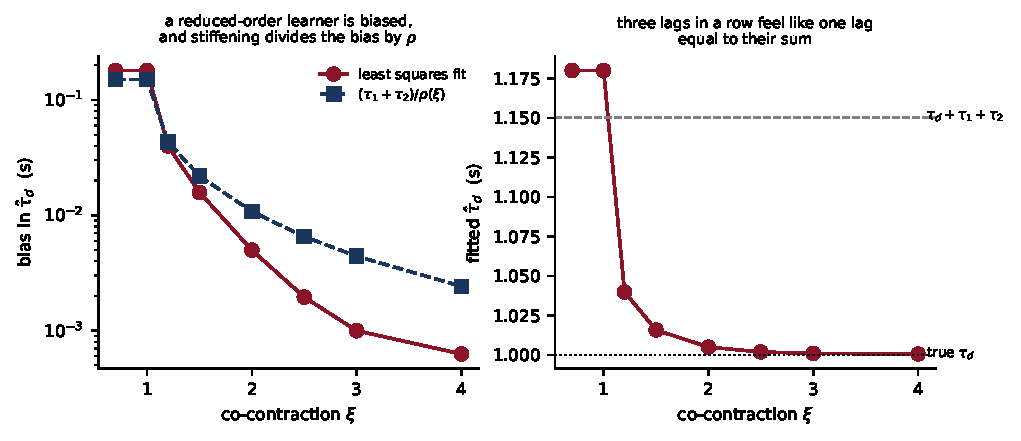
\includegraphics[width=\linewidth]{../outputs/learner2/bias_law.pdf}
  \caption{\textbf{Bias law, panel by panel.} \emph{Left panel}: bias in
    $\hat\tau_d$ plotted against $\xi$ on a log scale, comparing the actual
    least-squares fit (solid, circles) against the closed-form prediction
    $(\tau_1+\tau_2)/\rho(\xi)$ (dashed, squares). Both curves fall together
    from about 0.18\,s at $\xi=0.7$ toward well under a millisecond by
    $\xi=4$. The two curves tracking each other this closely across two
    decades of bias is the direct experimental confirmation of
    \eqref{eq:bias_law}. \emph{Right panel}: the fitted $\hat\tau_d$ itself
    (not the bias) plotted against $\xi$, together with two horizontal
    reference lines: the true $\tau_d=1.0$\,s (bottom) and the naive sum
    $\tau_d+\tau_1+\tau_2=1.15$\,s (top, the fully-soft prediction from
    \eqref{eq:bias_soft}). The fitted curve starts near the top line at low
    $\xi$ and descends smoothly toward the bottom line as $\xi$ increases,
    visually showing the learner's belief moving from ``systematically too
    slow'' to ``correct'' purely as a function of stiffness.}
  \label{fig:bias}
\end{figure}

\begin{examplebox}{Bias law, in one sentence}
You believe the cup has one time constant. With a soft arm you measure
$\approx1.18$\,s (close to the sum of all three true time constants). With a
very stiff arm ($\xi=4$) you measure $\approx1.0006$\,s, almost exactly the
true $1.0$\,s. Co-contraction did not change the cup at all --- it stopped the
fast, unmodelled parts of the cup's behaviour from leaking into, and
polluting, your \textbf{simple} one-parameter estimate of the slow part.
\end{examplebox}

% =============================================================================
\section{Part VI --- Learner 1 (gradient descent, order unlocked by hand)}
\label{sec:learner1}
% =============================================================================

\subsection{What it believes, and why that is the problem}

Learner~1 (code: \texttt{learner.py}, \texttt{experiment.py}) is a
\textbf{gray-box} learner: it is told the correct model structure, three lags
in series, and only has to find the right numbers $\hat\tau_d,\hat\tau_1,\hat\tau_2$
for them. Crucially, when it is only allowed to use $n_{\mathrm{unlocked}}\in\{1,2,3\}$
of the three parameters, the remaining ones are \textbf{forced to exactly zero}
(a pure pass-through, no lag at all), rather than being allowed to settle on
whatever value best explains the data. This single design choice, made before
the bias law of \S\ref{sec:bias} had been derived, is what prevents
Learner~1 from ever exhibiting that bias law: when $n_{\mathrm{unlocked}}=3$
(which happens in every condition eventually, since Learner~1's curriculum
always ends by unlocking all three parameters), the learner is
\textbf{correctly specified}, meaning it uses exactly the true model structure,
and a correctly specified least-squares fit converges to the true parameters
as more data arrive, with an error that is pure random noise, shrinking as
$1/\sqrt{N}$ in the number of trials $N$. There is no systematic bias left for
co-contraction to remove, because none was ever introduced.

Initial guesses before any learning: $\hat\tau=(0.30,\,0.03,\,0.015)$\,s ---
deliberately wrong, roughly three times too fast on every mode, so the learner
has real work to do.

\subsection{Prediction}

Given the command $u$ actually sent this trial and the stiffness $\xi$ chosen
for it, the learner's prediction is built the same way the true output is
built in \eqref{eq:output}, but using the learner's \emph{current beliefs}
$\hat\tau$ instead of the truth:
\begin{equation}
\hat y(t) = \text{cascade}\bigl(\text{felt}(\hat\tau,\xi), u\bigr).
\label{eq:pred1}
\end{equation}

\subsection{Learning rule: gradient descent}

\begin{techbox}{Gradient descent, from first principles}
\textbf{The goal.} We have a cost function $\mathcal C(q)$ (here, half the sum
of squared prediction errors, with $q=\log\hat\tau$ the parameters we control)
and we want the $q$ that makes $\mathcal C$ as small as possible.

\textbf{The idea.} The gradient $\nabla\mathcal C(q)$ is a vector that points
in the direction in which $\mathcal C$ increases \emph{fastest}. So $-\nabla
\mathcal C(q)$ points in the direction of \emph{steepest decrease}. Taking a
small step in that direction, and repeating, is guaranteed (for a small enough
step size $\eta$) to reduce $\mathcal C$ on every step, and to converge to a
point where the gradient is zero, i.e.\ a local minimum.

\textbf{Why it can be slow.} If the cost surface is shaped like a long, narrow
valley (some directions in parameter space change the cost a lot, others
barely at all --- this is exactly the situation \S\ref{sec:diag} below calls
``ill-conditioned''), plain gradient descent zig-zags slowly along the valley
floor instead of moving directly toward the minimum. This is the mathematical
reason ill-conditioning matters for a gradient learner, and it is used
explicitly in \S\ref{sec:diag}.
\end{techbox}

Concretely, the code keeps the residuals from the last 3 trials
(\texttt{BUFFER=3}) stacked together, $r=y-\hat y$ (all trials concatenated),
with cost $\mathcal C(q)=\tfrac12\sum_t r_t^2$. Parameters are stored in
\textbf{log} time constants, $q=\log\hat\tau$ (this keeps $\hat\tau$
automatically positive, and makes a fixed step size in $q$ correspond to a
fixed \emph{percentage} change in $\hat\tau$, which is fairer across modes
that differ by a factor of 20 in true magnitude).

\begin{stepbox}{From cost to update rule}
\textbf{Step 1.} By the chain rule, $\dfrac{\partial\mathcal C}{\partial
q_k}=\sum_t r_t\dfrac{\partial r_t}{\partial q_k}$. Writing this as a matrix
product with the \textbf{Jacobian} $J_{tk}=\partial r_t/\partial q_k$
(computed numerically by finite differences in the code, i.e.\ nudging each
$q_k$ by a tiny amount and seeing how much $r$ changes):
\[
\nabla\mathcal C = J^\top r.
\]

\textbf{Step 2.} Take a gradient-descent step with learning rate $\eta=3$,
averaged over the $m$ residual samples so the step size does not depend on
how much data happens to be in the buffer:
\begin{equation}
q \leftarrow q - \eta\,\frac{J^\top r}{m}.
\label{eq:gd}
\end{equation}

\textbf{Step 3.} Repeat \eqref{eq:gd} 12 times per trial
(\texttt{STEPS\_PER\_TRIAL=12}), recomputing $r$ and $J$ at the updated $q$
each time (this makes it closer to a proper Gauss--Newton-style fit within
each trial, while still being called ``gradient descent'' because the
underlying update direction is the gradient).
\end{stepbox}

\subsection{Conditions S1--S5}

\begin{center}
\small
\begin{tabular}{@{}llp{6.5cm}@{}}
\toprule
\textbf{Code} & \textbf{Tuning schedule} & \textbf{What is imposed} \\
\midrule
S1 & soft, fast, 3 modes unlocked from trial 1 & the ``deep end'' \\
S2 & $\xi:3\to1.3\to0.7$, slow$\to$fast, unlock $1\to2\to3$ & the Thrish curriculum \\
S3 & stiff throughout, 1 mode only, forever & never allowed to learn transients \\
S4 & soft throughout, only speed staged, unlock $1\to2\to3$ & tests the speed channel alone \\
S5 & random $\xi$ drawn fresh every trial & control for mere variability \\
\bottomrule
\end{tabular}
\end{center}

The stage-advance rule for S2 and S4 (\texttt{\_maybe\_advance}) moves to the
next stage once at least \texttt{MIN\_TRIALS\_PER\_STAGE}=6 trials have been
run \emph{and} the prediction error has stopped improving for
\texttt{PLATEAU\_STREAK}=2 consecutive trials --- i.e.\ the schedule advances
when the current stage's learning has plateaued, not on a rigid trial count.

\subsection{Results (20 seeds, 80 trials) and why they refute the speed claim}
\label{sec:learner1results}

\begin{warnbox}{Learner~1 refuted the ``curriculum learns faster'' claim}
\begin{center}
\begin{tabular}{@{}lrrrr@{}}
\toprule
 & median trials to criterion & reached criterion & final error & failed trials \\
\midrule
S1 deep end & 47 & 100\% & 0.043 & 10.4 \\
S2 curriculum & 80 & 55\% & 0.105 & 0.0 \\
S3 stiff forever & --- (never) & 0\% & 0.439 & 0.0 \\
S4 bandwidth only & 70 & 100\% & 0.084 & 11.55 \\
S5 random & --- (never) & 0\% & 0.233 & 0.95 \\
\bottomrule
\end{tabular}
\end{center}
S2 needed a \textbf{median 33 trials more} than S1 to reach the same criterion
(two-sided Mann--Whitney with Holm correction, $p\approx1.6\times10^{-7}$).
The curriculum won decisively on \textbf{safety} (zero failed trials versus
10.4 for S1), but lost on speed.
\end{warnbox}

\subsubsection{Two diagnostic facts that explain why}
\label{sec:diag}

Both computed by \texttt{diagnose.py}, using the curvature (information)
matrix $H^\top H$ evaluated at the true parameters (see \S\ref{sec:metrics}
for the exact definition of $\kappa$).

\begin{enumerate}[nosep]
\item \textbf{Co-contraction makes the full three-parameter fit harder, not
  easier, to identify.} The condition number $\kappa(\Phi)$ of the
  information matrix for the \emph{complete} three-mode fit rises from about
  $5.5\times10^3$ when soft ($\xi=0.7$) to about $1.8\times10^{16}$ when stiff
  ($\xi=3$) --- an increase of \textbf{thirteen orders of magnitude}. Over the
  same range, the curvature on just the dominant mode's own parameter only
  improves from $2.54\times10^{-2}$ to $2.72\times10^{-2}$: about 7\%. Stiffening
  buys almost nothing for the direction that matters, while making the other
  two directions almost invisible to the data (this is exactly the analytic
  content of \eqref{eq:bias_law}, seen from a different angle: the fast modes'
  information about themselves vanishes, but --- for a learner that
  \emph{must} fit them, as Learner~1 eventually must --- vanishing information
  about a required parameter is bad, not good).

\item \textbf{The parameter directions that are hardest to learn are also the
  ones that matter least behaviourally.} Taking equal-sized steps along each
  eigenvector of the curvature matrix and measuring how much the resulting
  impulse response changes, the direction with the smallest curvature (i.e.\
  slowest to learn, by a factor of about 5500$\times$ relative to the largest)
  changes behaviour by only about 28$\times$ less than the best-conditioned
  direction. In other words, exactly the directions the sample-complexity
  bound $N(r,\delta)\propto \sigma^2 r/(\delta\lambda_{\min}(\Phi_r))$ (see the
  meeting note, \texttt{meetings/2026-07-01-meeting-thrish.tex}) says are expensive
  to estimate precisely are the directions whose imprecision costs the least
  in terms of actual behaviour. This is why a bound on \emph{parameter} error
  does not translate into a bound on \emph{behavioural} error, and it is the
  single technical reason the ``order reduction buys faster learning''
  argument, as originally stated, does not survive contact with an
  identification problem that is correctly specified.
\end{enumerate}

\begin{figure}[ht]
  \centering
  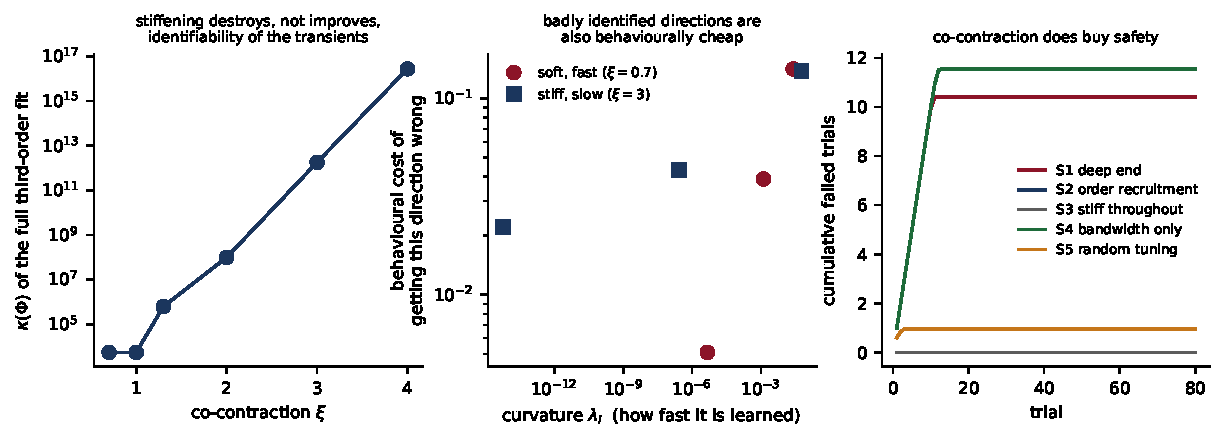
\includegraphics[width=\linewidth]{../outputs/curriculum/mechanism.pdf}
  \caption{\textbf{Learner~1 diagnostics, panel by panel.} \emph{Left panel}:
    $\kappa(\Phi)$ for the full three-parameter fit, plotted against $\xi$ on
    a log scale. The line rises steeply and monotonically: stiffening steadily
    destroys the identifiability of the complete model, contrary to the naive
    expectation that a ``simpler-looking'' system should be easier to fit in
    full. \emph{Centre panel}: for each eigen-direction of the curvature
    matrix, curvature (x-axis, how fast that direction is learned) plotted
    against behavioural cost (y-axis, how much the impulse response changes
    if that direction is wrong by a fixed amount), both on log scales, for two
    stiffness levels. The points line up along a rising diagonal trend: low
    curvature (slow to learn) systematically pairs with low behavioural cost
    (does not matter much), for both stiffness levels. \emph{Right panel}:
    cumulative number of failed trials over the 80-trial run, one curve per
    condition. S1 and S4 climb quickly to roughly 10--12 failures and then
    flatten (once the model becomes good enough that the tolerance in
    \eqref{eq:tolerance} is no longer crossed); S2 and S3 stay at exactly zero
    throughout, because they never risk a soft, fast, badly-modelled reach.}
  \label{fig:mech1}
\end{figure}

% =============================================================================
\section{Part VII --- Learner 2 (two-timescale EKF + ARD)}
\label{sec:learner2}
% =============================================================================

Learner~2 (code: \texttt{kalman\_learner.py}, \texttt{experiment2.py}) is
built to remove both defects identified above:
\begin{enumerate}[nosep]
\item \textbf{Misspecification.} Learner~1 always used the true three-lag
  structure whenever a mode was unlocked, so it could never exhibit the bias
  law \eqref{eq:bias_law}. Learner~2 always carries \emph{all three} modes,
  but lets each transient mode's \emph{participation} in the prediction vary
  continuously between ``fully present'' and ``not present'', so it can
  genuinely behave as a lower-order model when the data do not support more.
\item \textbf{Overconfidence about the unobservable.} A fixed-step learner
  that receives essentially no information about a mode (because it is
  stiffened away) still takes fixed-size steps on that mode's parameter,
  driven purely by noise --- a \textbf{random walk} that can destroy a
  perfectly good previous estimate. Learner~2 tracks its own
  \textbf{uncertainty} explicitly, so that a parameter direction with no
  information in the current data is simply left alone rather than perturbed.
\end{enumerate}

\subsection{State vector}

\begin{equation}
q = \bigl[\log\hat\tau_d,\ \log\hat\tau_1,\ \log\hat\tau_2,\ w_1,\ w_2\bigr]^\top.
\label{eq:state2}
\end{equation}

The first three entries are the same log-time-constants as Learner~1. The two
new entries, $w_1,w_2\in[0,1.2]$, are \textbf{participation weights}: real
numbers (not switches) describing how much of each transient mode is
currently included in the learner's own prediction.

\subsection{Blend dynamics: why not just set $\tau=0$?}

Rather than removing a mode by literally setting its time constant to zero
(which is what ``locking'' a mode meant for Learner~1), each transient mode's
lag is \textbf{blended} with a pass-through, in proportion $w$:
\begin{equation}
\mathrm{blend}(\tau,w)[x] = (1-w)\,x + w\cdot\mathrm{lag}(\tau)[x].
\label{eq:blend}
\end{equation}

\begin{itemize}[nosep]
\item At $w=1$: $\mathrm{blend}=\mathrm{lag}(\tau)[x]$, the mode is fully
  present, exactly as in Learner~1.
\item At $w=0$: $\mathrm{blend}=x$, the mode contributes nothing to the
  prediction, matching what ``mode absent'' should mean --- \emph{but} the
  formula still contains $\tau$ and $w$ as adjustable quantities, so the
  \emph{sensitivity} of the prediction to a small change in $w$ (its partial
  derivative) is not zero even when $w$ itself is zero.
\end{itemize}

\begin{stepbox}{Checking that the derivative survives at $w=0$}
Differentiate \eqref{eq:blend} with respect to $w$:
\[
\frac{\partial}{\partial w}\Bigl[(1-w)x + w\cdot\mathrm{lag}(\tau)[x]\Bigr]
= -x + \mathrm{lag}(\tau)[x] = \mathrm{lag}(\tau)[x] - x.
\]
This does not depend on the current value of $w$ at all --- it is the same
nonzero quantity (as long as $\mathrm{lag}(\tau)[x]\ne x$, i.e.\ the lag
actually does something) whether $w$ is currently 0, 0.5, or 1. So the
gradient-based filter always has \emph{some} signal telling it whether to
raise or lower $w$, even from a starting point of exactly zero.
\end{stepbox}

\begin{examplebox}{Volume knobs versus deleting a mode entirely}
Wrong approach (what an earlier attempt at Learner~2 did, and which had to be
fixed): encode ``mode off'' by setting $\hat\tau_2=0$ directly. Then the
model's output literally does not depend on $\hat\tau_2$ at that point ---
its derivative is exactly zero --- so once the fast mode is switched off while
stiff, no future data, however clearly it shows the transient during a later
soft trial, can ever switch $\hat\tau_2$ back on. Pruning becomes
\textbf{irreversible}, which contradicts the very phenomenon (relaxing later
to learn the transient) the simulation is meant to demonstrate.

Right approach (what the code actually does): encode ``mode off'' by setting
the \emph{weight} $w_2=0$ instead, leaving $\hat\tau_2$ itself free. The
derivative with respect to $w_2$ stays alive at $w_2=0$ (as just shown), so
when soft, fast data eventually arrive and strongly favour a nonzero fast
mode, $w_2$ can rise again in response. Pruning is \textbf{reversible}.
\end{examplebox}

The full prediction chain, applying \eqref{eq:blend} twice after the always-on
dominant lag (code: \texttt{kalman\_learner.\_h}):
\begin{align}
x_0 &= \mathrm{lag}(\hat\tau_d)[u] \nonumber\\
x_1 &= \mathrm{blend}\bigl(\hat\tau_1/\rho(\xi),\, w_1\bigr)[x_0] \nonumber\\
\hat y &= \mathrm{blend}\bigl(\hat\tau_2/\rho(\xi),\, w_2\bigr)[x_1]
\label{eq:chain2}
\end{align}

\subsection{Effective order}

\begin{equation}
\boxed{\;\neff = 1 + w_1 + w_2\;}
\label{eq:neff}
\end{equation}

This is exactly the ``effective order'' quantity the meeting note makes its
central observable, made concrete: it is simply the sum of the dominant mode
(always fully present, contributing 1) plus however much of each transient
mode the learner currently believes is real. It is never set by hand in the
code; it is read off the current weights, which are themselves determined by
the filter and the ARD mechanism below.

% ---------------------------------------------------------------------------
\subsection{Extended Kalman Filter (EKF) --- full derivation from Bayes' rule}
\label{sec:ekf}
% ---------------------------------------------------------------------------

\begin{techbox}{Why a Kalman filter, from the ground up}
\textbf{The problem.} We have a belief about the unknown parameters $q$, and
each trial we get a noisy measurement that depends on $q$ nonlinearly through
\eqref{eq:chain2}. We want a principled way to (a) update the belief using the
new data, and (b) keep track of \emph{how confident} we should be, so a
parameter with no information in the data is correctly left uncertain rather
than being nudged around by noise.

\textbf{The Bayesian starting point.} Represent the belief as a Gaussian
distribution over $q$: mean $\hat q$ (the current best guess) and covariance
$P$ (how spread out, i.e.\ uncertain, the belief is in every direction).
Before seeing new data, let the belief drift by adding process noise $Q$ (this
models the idea that the true parameters, or at least our confidence about
them, can change slightly from trial to trial):
\[
P_{\mathrm{pred}} = P + Q.
\]

\textbf{Combining a Gaussian prior with a Gaussian likelihood.} If the prior
on $q$ is Gaussian with covariance $P_{\mathrm{pred}}$, and the new
measurement $y$ is $y=h(q)+\text{noise}$ with noise variance $R$, then Bayes'
rule for Gaussians says the posterior is Gaussian with \textbf{precision}
(inverse covariance) equal to the sum of the prior's precision and the
measurement's precision, weighted by how sensitive $h$ is to $q$ (its
Jacobian $H$):
\[
P_{\mathrm{post}}^{-1} = P_{\mathrm{pred}}^{-1} + \frac{H^\top H}{R}.
\]
This is the core Kalman-filter idea, and it is exactly analogous to how
combining two independent noisy measurements of the same quantity gives a
combined estimate with smaller variance than either alone: precisions simply
add.

\textbf{Nonlinearity.} Because \eqref{eq:chain2} is nonlinear in $q$
(it passes $u$ through exponentials of $q$), we cannot apply the Gaussian
update exactly. The \textbf{Extended} Kalman Filter (EKF) approximates the
nonlinear function by its \textbf{first-order Taylor expansion} (i.e.\ its
tangent plane) around the current best guess, computes the update as if that
linear approximation were exact, and then --- because a single linearisation
around a possibly-still-wrong guess can itself introduce error --- the code
repeats this linearise-and-update step three times per trial (an
\textbf{iterated} EKF), re-linearising around the improved guess each time.
\end{techbox}

\subsubsection{Setting up the linearisation}

Write $h(q)=\eqref{eq:chain2}$ evaluated at parameters $q$, for the whole
trial's worth of samples at once, so $h(q)$ is a vector of predicted samples.
The measurement error and its sensitivity to $q$ are:
\begin{equation}
e = y - h(q),\qquad H = \left.\frac{\partial h}{\partial q}\right|_{q}.
\label{eq:lin}
\end{equation}
$H$ is computed numerically in the code by finite differences: nudge each
entry of $q$ by a tiny amount $10^{-3}$, re-run $h$, and divide the change in
output by the nudge size.

\subsubsection{The information-form update, derived step by step}

\begin{stepbox}{From the Bayesian combination rule to the code}
\textbf{Step 1 (precision of the posterior).} As derived above, combine the
predicted precision $P_{\mathrm{pred}}^{-1}$, the measurement precision
$H^\top H/R$, and --- because the participation weights carry an extra prior
pulling them toward a target value (the ARD prior of \S\ref{sec:ard}) --- an
additional term $\diag(\alpha)$ representing that extra prior's precision:
\begin{equation}
A = P_{\mathrm{pred}}^{-1} + \frac{H^\top H}{R} + \diag(\alpha).
\label{eq:inf_A}
\end{equation}

\textbf{Step 2 (posterior covariance).} Invert to get the new covariance:
\begin{equation}
P_{\mathrm{post}} = A^{-1}.
\label{eq:inf_post}
\end{equation}

\textbf{Step 3 (posterior mean).} The posterior mean shift is the posterior
covariance times the sum of all the ``pulls'' on $q$: the pull from the
measurement error ($H^\top e/R$, ``move toward what explains the data''), the
pull from the ARD prior ($-\alpha(q-q_{\mathrm{target}})$, ``move toward the
prior's preferred value, in proportion to how strongly the prior believes in
it''), and the pull from the process-noise prior linking back to the previous
belief ($-P_{\mathrm{pred}}^{-1}(q-q_{\mathrm{pred}})$, ``don't drift
arbitrarily far from where you started this trial''):
\begin{equation}
q \leftarrow q + P_{\mathrm{post}}\left(\frac{H^\top e}{R}
  - \alpha(q-q_{\mathrm{target}})
  - P_{\mathrm{pred}}^{-1}(q-q_{\mathrm{pred}})\right).
\label{eq:inf_update}
\end{equation}

\textbf{Step 4 (why this is the same as the textbook Kalman gain form).}
Equations \eqref{eq:inf_A}--\eqref{eq:inf_update} are the ``information
form'' of the Kalman update. It is mathematically equivalent to the more
commonly seen form written with an explicit ``Kalman gain'' matrix $K_{\mathrm{gain}}
=P_{\mathrm{pred}}H^\top(HP_{\mathrm{pred}}H^\top+R)^{-1}$ and update $q
\leftarrow q_{\mathrm{pred}}+K_{\mathrm{gain}}e$; the information form is used
here because it lets the extra ARD precision term $\diag(\alpha)$ be added in
directly, without needing a separate ``pseudo-measurement'' trick.
\end{stepbox}

\subsubsection{Why $R$ is inflated during early trials}

If $R$ (the measurement noise variance) were fixed at the true sensor-noise
level, the filter would treat \emph{all} of the residual $e$ as informative
about $q$, even in early trials when most of the residual is actually caused
by the model still being wrong, not by sensor noise. The code instead sets
\[
R = \max\bigl(R_{\mathrm{std}}^2,\ \mathrm{mean}(e^2)\bigr),
\]
so that while the fit is still poor, $R$ is large (the filter treats the
measurement as unreliable and updates cautiously); once the residual shrinks
close to the true noise floor, $R$ settles back to $R_{\mathrm{std}}^2$ and
the filter becomes appropriately confident.

\begin{examplebox}{EKF, worked through one trial}
Day 1: the learner's guess for the cup's main time constant is 0.3\,s, and it
is very unsure ($P_{11}$ large). It makes a slow, stiff reach and feels a
sluggish response. The prediction error $e$ is large and mostly explained by
$\hat\tau_d$ being too small, so $H^\top e/R$ points strongly in the direction
of increasing $\hat\tau_d$; the update in \eqref{eq:inf_update} moves the
estimate toward roughly 0.8\,s and \eqref{eq:inf_post} shrinks the
uncertainty $P_{11}$ accordingly. Meanwhile, because the reach was stiff, the
columns of $H$ corresponding to $w_1,w_2$ are nearly zero (the fast modes
contributed almost nothing to $\hat y$, per \eqref{eq:felt}), so the
corresponding rows and columns of $H^\top H/R$ are nearly zero too, and those
uncertainties barely shrink. The learner correctly ``knows that it does not
yet know'' about the transients.
\end{examplebox}

% ---------------------------------------------------------------------------
\subsection{ARD --- Automatic Relevance Determination, derived}
\label{sec:ard}
% ---------------------------------------------------------------------------

\begin{techbox}{ARD, from first principles}
\textbf{The idea.} We want each participation weight $w_i$ to be pulled toward
zero (``this mode probably does not matter'') \emph{unless} the data
consistently push back against that pull. This is achieved with a Gaussian
prior on $w_i$ centred at $0$ with precision $\alpha_i$: the larger $\alpha_i$,
the more strongly $w_i$ is pulled toward zero, and the smaller its allowed
range of movement.

\textbf{The trick: let the data set $\alpha_i$ itself.} Rather than fixing
$\alpha_i$ by hand, ARD updates it after every trial based on how well
determined $w_i$ currently is. Define $\gamma_i=1-\alpha_i P_{ii}$, a quantity
between 0 and 1 that measures how much of $w_i$'s current uncertainty $P_{ii}$
is explained by \emph{data} rather than by the prior alone (when the prior
dominates, $\alpha_iP_{ii}\to1$ so $\gamma_i\to0$; when data dominate,
$\alpha_iP_{ii}\to0$ so $\gamma_i\to1$). Then update:
\begin{equation}
\alpha_i \leftarrow \frac{\gamma_i}{\max(w_i^2,\varepsilon)}.
\label{eq:ard}
\end{equation}

\textbf{Why this produces automatic pruning.} If the data do not support mode
$i$ (its estimate $w_i$ stays small and uncertain), $\gamma_i$ stays away from
1 while $w_i^2$ in the denominator is small, so $\alpha_i$ does not blow up
uncontrollably (it is capped in the code, \texttt{ALPHA\_BOUNDS}, precisely so
that pruning stays reversible rather than permanent) but stays large enough to
keep pulling $w_i$ toward zero. If instead the data strongly support a
sizeable $w_i$, then $w_i^2$ in the denominator grows, driving $\alpha_i$ down
and \emph{releasing} the pull, letting $w_i$ settle wherever the data actually
want it.
\end{techbox}

This is precisely how $\neff$ in \eqref{eq:neff} falls toward 1 while stiff
(the transients have no data to justify keeping their weights up, so ARD
shrinks them) and rises again once co-contraction relaxes and soft, fast
trials start to supply real information about the transients --- without a
single line of code anywhere saying ``unlock mode 2 now''.

\subsection{Two timescales}

Process noise on the state (\texttt{PROCESS\_NOISE}, roughly):
\[
Q = \diag\bigl(10^{-5},\ 2\times10^{-3},\ 2\times10^{-3},\ 2\times10^{-3},\ 2\times10^{-3}\bigr).
\]
The dominant log-time-constant is allowed to drift 200 times more slowly than
everything else. This is the concrete implementation of the ``two-timescale''
idea: a slow, well-retained channel for the part of the model that matters
across the whole learning process, and a fast, more forgetful channel for the
parts that are only relevant once they have been exposed by relaxing.

\subsection{Conditions K1--K5}

Identical tuning schedules to S1--S5, but with two crucial differences from
Learner~1's setup:
\begin{itemize}[nosep]
\item \textbf{No hand-imposed unlocking.} All three $\hat\tau$'s and both
  weights $w_1,w_2$ exist from trial one in every condition, including K3
  (stiff throughout). Whatever effective order K3 ends up at is discovered by
  the filter, not decided in advance by the code.
\item \textbf{Confidence-gated relaxation for K2 and K4.} Rather than
  advancing on a fixed trial count, the schedule advances once the
  posterior standard deviation of $\log\hat\tau_d$ falls below a threshold
  (\texttt{CONFIDENCE\_SD}=0.04): the learner relaxes only once it is
  genuinely confident about the part of the model it can currently see, which
  is the direct computational version of Thrish's ``learn that, then relax a
  little bit more''.
\end{itemize}

\subsection{Results (20 seeds, 60 trials) and what each number means}
\label{sec:learner2results}

\begin{resultbox}{Learner~2 confirms the mechanism; still does not confirm the speed claim}
\begin{center}
\begin{tabular}{@{}lrrrrr@{}}
\toprule
 & trials to criterion & final error & peak $|\hat\tau_d-\tau_d|$ & final $\neff$ & failed trials \\
\midrule
K1 deep end & 5 & 0.031 & 0.691\,s & 2.18 & 4.0 \\
K2 confidence-gated & 19 & 0.030 & 0.087\,s & 2.18 & 0.0 \\
K3 stiff forever & --- (never) & 0.404 & 0.013\,s & 1.00 & 0.0 \\
K4 bandwidth only & 4 & 0.030 & 0.026\,s & 2.19 & 1.1 \\
K5 random & 35 & 0.076 & 0.040\,s & 1.92 & 0.7 \\
\bottomrule
\end{tabular}
\end{center}
\end{resultbox}

\begin{figure}[ht]
  \centering
  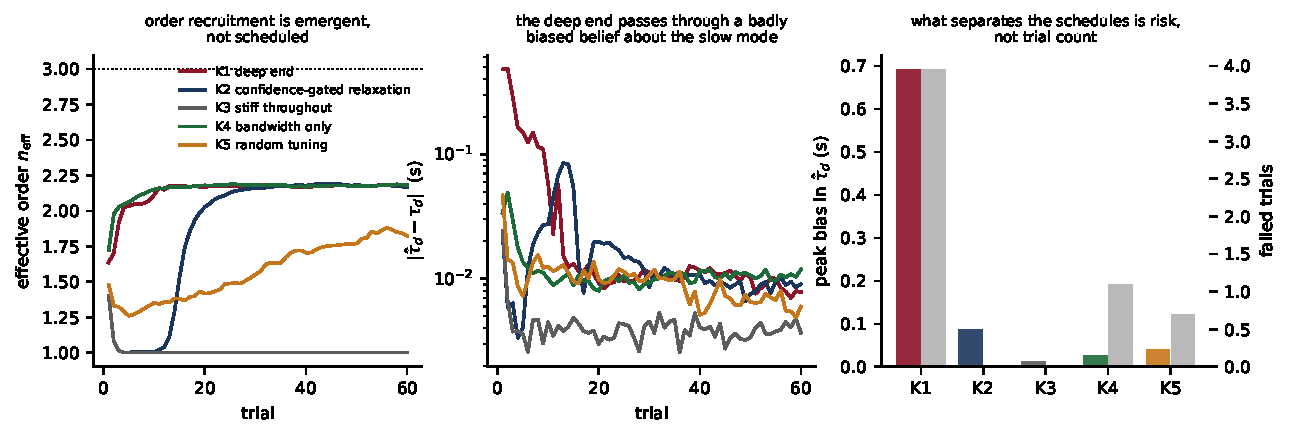
\includegraphics[width=\linewidth]{../outputs/learner2/learner2.pdf}
  \caption{\textbf{Learner~2, panel by panel.} \emph{Left panel}: $\neff$
    (\eqref{eq:neff}) plotted against trial number for all five conditions.
    K3 (stiff throughout) drops to and holds exactly at $\neff=1.00$ for the
    entire run: the learner has discovered, purely from ARD shrinking $w_1$
    and $w_2$ toward zero, that it should behave as a first-order system, with
    no rule anywhere telling it to. K2 tracks K3 closely at $\neff\approx1$
    while stiff, then rises sharply to about $2.2$ at the exact trial where
    the confidence-gated schedule permits relaxation (\S sect. on K1--K5
    above): this is progressive order recruitment happening as a consequence
    of the ARD mechanism responding to newly available data, not because a
    schedule told it to. K1 and K4, which never restrict themselves at all,
    rise to $\neff\approx2.2$ almost immediately. \emph{Centre panel}: the
    absolute error $|\hat\tau_d-\tau_d|$ over trials, log scale. K1's curve
    starts at roughly $0.1$ and briefly rises to nearly $0.7$ before falling
    --- this transient overshoot, entirely absent from K3, is the
    misspecification bias of \eqref{eq:bias_law} being incurred and then paid
    off as the learner is exposed to all three modes simultaneously while
    still uncertain. K2's curve stays low throughout the stiff stage and only
    shows a much smaller bump around the trial where it relaxes.
    \emph{Right panel}: a bar chart with two axes, peak bias (coloured bars,
    left axis) and number of failed trials (grey bars, right axis), one pair
    per condition. K1 has both the largest peak bias and the most failures;
    K2 and K3 both have essentially zero failures, with K2's peak bias
    (from the same brief transient period visible in the centre panel) still
    roughly 8 times smaller than K1's. This panel is the clearest single
    visual statement of the paper's actual finding: \textbf{the schedules
    differ in the risk incurred while learning, not in how many trials
    learning takes.}}
  \label{fig:learner2}
\end{figure}

\begin{examplebox}{Reading K2 versus K1, side by side}
Both K1 and K2 end up at essentially the same final model
(error $\approx0.03$, $\neff\approx2.2$). K1 gets there in only about 5
trials, but along the way its belief about the dominant time constant is, at
its worst point, wrong by about $0.7$\,s --- nearly as large as the true value
itself --- and 4 of its trials fail outright (the ``ball goes out''). K2 takes
roughly four times as many trials (about 19) to reach the same final model,
but its worst-case error in the dominant time constant is only about
$0.09$\,s, and it never once fails a trial. In other words: \textbf{the
curriculum buys a much safer route to the same destination, not a shorter
one.}
\end{examplebox}

% =============================================================================
\section{Part VIII --- Scoring metrics (every formula, fully explained)}
\label{sec:metrics}
% =============================================================================

\textbf{Relative impulse error} --- the headline measure of ``how wrong is the
learned object model, overall?'' Simulate an impulse (a very brief, very
strong pulse) through both the true object and the learner's current belief
about the object, and compare the two resulting responses:
\begin{equation}
\mathrm{err} = \frac{\|y_{\mathrm{imp}}-\hat y_{\mathrm{imp}}\|_2}{\|y_{\mathrm{imp}}\|_2},
\qquad \|v\|_2 = \sqrt{\textstyle\sum_k v_k^2}.
\label{eq:imperr}
\end{equation}
This is zero only if the learner's belief produces \emph{exactly} the same
impulse response as the truth at every time sample, and it is normalised by
the size of the true response so that a value of, say, $0.1$ means ``the
model's error is about 10\% of the size of the true signal'', regardless of
the absolute scale of the signal.

\textbf{Trials to criterion} --- the first trial number at which
$\mathrm{err}<0.10$ for 3 consecutive trials in a row (a ``streak'', so a
single lucky trial does not count as having converged).

\textbf{Condition number} $\kappa(\Phi)$ (Learner~1 diagnostics, computed by
\texttt{diagnose.py}). Form the curvature (information) matrix
$\Phi=H^\top H$ from the Jacobian $H$ of the prediction with respect to the
(log) parameters, evaluated at the true parameter values. This matrix has
three eigenvalues $\lambda_1\ge\lambda_2\ge\lambda_3\ge0$ (since $\Phi$ is
symmetric positive semi-definite), each with an associated eigenvector
telling you a direction in parameter space. The condition number is the ratio
of the largest to the smallest:
\begin{equation}
\kappa(\Phi) = \frac{\lambda_1}{\lambda_3}.
\label{eq:kappa}
\end{equation}

\begin{stepbox}{Why a large $\kappa$ means ``some directions are invisible''}
\textbf{Step 1.} The eigenvalue $\lambda_i$ measures how much the sum of
squared prediction errors changes if you move a unit distance along
eigen-direction $i$: a large $\lambda_i$ means moving that way changes the
predictions a lot (easy to detect from data), a small $\lambda_i$ means moving
that way changes the predictions very little (hard to detect).

\textbf{Step 2.} If $\lambda_1/\lambda_3$ is enormous (as it is for the stiff
conditions, $\sim10^{16}$), then direction 3 changes the predictions by a
factor of $10^{16}$ less than direction 1 does. Any realistic amount of
measurement noise will completely swamp whatever tiny signal exists about
direction 3, making that parameter combination effectively unidentifiable
from the available data.
\end{stepbox}

% =============================================================================
\section{Learner 4 --- co-contracting in order to learn}
\label{sec:learner4}
% =============================================================================

Learners~1--3 scored a model of the \emph{whole object}. That is why the stiff
first-order conditions (S3, K3, C3) looked like failures: their impulse error
against the true third-order cup plateaus near $0.40$, even when
$\hat\tau_d$ is essentially perfect. Learner~4 changes the
\emph{scoreboard}, not the plant, and puts the three strategies a person
could actually adopt side by side:

\begin{enumerate}[nosep]
\item \textbf{Do not co-contract}, and identify the whole third-order plant.
\item \textbf{Co-contract and learn only the slow lag}, treating the
  transients as noise.
\item \textbf{Co-contract, then relax progressively} and learn the whole
  model gradually.
\end{enumerate}

The underlying claim is that the third strategy should dominate, because
without co-contraction the learner faces a third-order identification
problem, whereas with it the coupling has already filtered the transients
and the learner faces a first-order one.

Movement time is held at the fast reach ($t_{\mathrm{move}}=0.25$\,s) in
\emph{every} cell, including the staged ones, so the only quantity that ever
varies is $\xi$.

\begin{center}
\small
\begin{tabular}{@{}llll@{}}
\toprule
 & Learner & $\xi$ & Strategy \\
\midrule
L1 & third-order EKF & $0.7$ & no co-contraction, learn the full model \\
L2 & first-order EKF on $\log\tau_d$ & $3.0$ & co-contract, learn the slow model only \\
L3 & first-order EKF on $\log\tau_d$ & $0.7$ & control: capacity without the filter \\
L4 & third-order EKF & $3.0$ & control: filter without the restriction \\
L5 & third-order EKF & staged & co-contract, then learn the whole model gradually \\
L6 & first $\to$ third-order & staged & learn the slow lag stiff, then warm-start \\
\bottomrule
\end{tabular}
\end{center}

\subsection{Guide to the six conditions (L1--L6)}
\label{sec:learner4guide}

Table~\ref{tab:learner4conditions} is the lay reference for every row in
Figure~\ref{fig:learner4}.  L1, L2 and L5 are the three strategies a person
could actually adopt; L3 and L4 are \emph{controls} that isolate which half
of L2 is doing the work; L6 is the strongest version of the staged
hypothesis.

\small
\begin{longtable}{@{}p{0.7cm}p{1.5cm}p{2.0cm}p{2.2cm}p{4.8cm}p{2.6cm}@{}}
\caption{What each Learner~4 condition means, with an everyday cup-and-arm
example.  Movement speed is the same fast reach in every row; only
co-contraction $\xi$ and the learner's model capacity differ.}
\label{tab:learner4conditions}\\
\toprule
\textbf{Code} & \textbf{Co-contraction} & \textbf{Learner capacity} & \textbf{Strategy in one line} &
\textbf{Everyday example (cup of coffee)} & \textbf{Role} \\
\midrule
\endfirsthead
\toprule
\textbf{Code} & \textbf{Co-contraction} & \textbf{Learner capacity} & \textbf{Strategy in one line} &
\textbf{Everyday example (cup of coffee)} & \textbf{Role} \\
\midrule
\endhead
L1 &
Soft throughout ($\xi=0.7$) &
Full third-order (three lags) &
No co-contraction: learn the whole cup from trial one &
You pick up a full mug with a \emph{relaxed} arm and try to learn
\emph{everything at once}---how sluggish the cup feels \emph{and} how it
wobbles and sloshes.  Fast, but you spill sometimes while your mental model
is still wrong. &
Main comparison: the ``deep end'' \\
\addlinespace
L2 &
Stiff throughout ($\xi=3.0$) &
Slow only (one lag, $\tau_d$) &
Co-contract and learn only the slow part; treat wobble as filtered out &
You \emph{squeeze hard} the whole time and tell yourself: ``I only need to
learn how \emph{heavy/sluggish} this cup is; the quick slosh is not in what
I feel.''  You learn that sluggishness in three trials and never spill---but
you never learn the slosh because you never relax. &
Human-like slow-only strategy \\
\addlinespace
L3 &
Soft throughout ($\xi=0.7$) &
Slow only (one lag) &
\emph{Control:} same capacity as L2, but \emph{no} filter &
You use the same ``only learn sluggishness'' mindset as L2, but your arm
stays \emph{soft}, so the slosh is still plainly there.  Ignoring it is
now a \emph{mistake}, not a filter: you merge wobble into your sluggishness
estimate, stay systematically wrong, and keep spilling. &
Negative control for L2 \\
\addlinespace
L4 &
Stiff throughout ($\xi=3.0$) &
Full third-order (three lags) &
\emph{Control:} full capacity, filter present, never relax &
You squeeze hard and your brain \emph{could} track three time scales---but
while stiff the fast ones vanish from the data, so the learner \emph{prunes
itself} to first order anyway ($\neff=1$).  Identical to L2 on the slow
scoreboard. &
Is the speed-up the filter or the restriction? \\
\addlinespace
L5 &
Staged: $3.0\to1.3\to0.7$ &
Full third-order &
Co-contract first, then relax when confident and learn the whole cup &
Thrish's curriculum: start with a \emph{stiff, braced} arm and learn safely;
once you are confident about the main sluggishness, \emph{relax in stages}
and let the slosh reappear so you can learn it too.  Zero spills; takes
longer than L1 if spills are free. &
Staged full-model strategy \\
\addlinespace
L6 &
Staged: $3.0\to1.3\to0.7$ &
Slow while stiff, then \emph{promoted} to full third-order &
Learn $\tau_d$ while stiff, then \emph{hand it over} to a full learner &
Same staging as L5, but the moment you first relax you \emph{transfer} your
slow-lag estimate (and how sure you are of it) into a fresh full-order
learner instead of making it rediscover sluggishness from scratch.  Best
compromise between safety and eventual full-cup knowledge. &
Strongest staged hypothesis \\
\bottomrule
\end{longtable}
\normalsize

\begin{examplebox}{How to read the three strategy rows}
\textbf{L1} asks: ``What if I never co-contract?''\;
\textbf{L2} asks: ``What if I co-contract and only keep the slow part?'';
\textbf{L5/L6} ask: ``What if I co-contract first and then learn the rest?''
The controls L3 and L4 answer \emph{why} L2 works when it does: L3 shows
that ignoring transients without a filter fails; L4 shows that the filter,
not the choice to use a one-parameter model, is what makes the slow lag
learnable in three trials.
\end{examplebox}

The first-order filter is the iterated-EKF step of \S\ref{sec:learner2},
restricted to the dominant-mode channel and with the same hyperparameters on
that channel, so L2 versus L1 is a comparison of \emph{what is being
estimated}, not of how the estimator works. The plant is unchanged: the two
fast lags are still there, and they are still compressed by $\rho(\xi)$.
Staged conditions relax through $\xi = 3.0 \to 1.3 \to 0.7$ under the same
confidence gate K2 used (posterior sd on $\log\tau_d$ below $0.04$, minimum
five trials per stage). L6 promotes at the first relaxation, transferring
$\log\tau_d$ and its posterior variance into a fresh third-order learner and
nothing else, so its head start is on the slow lag alone.

% ---------------------------------------------------------------------------
\subsection{One trial, line by line (lay walkthrough of \texttt{experiment4.py})}
\label{sec:learner4trial}
% ---------------------------------------------------------------------------

This subsection is the companion to the code in
\texttt{order\_reduction/experiment4.py}, function \texttt{run\_seed},
roughly lines 271--321.  Read it as a story: \emph{you pick up a cup, move
your hand, feel what happens, compare that to what your brain expected, and
(if you did not spill) update your mental model}.

\begin{howto}{Map of one trial (keep this picture in mind)}
\begin{center}
\small
\begin{tabular}{@{}cll@{}}
\toprule
\textbf{Step} & \textbf{Code} & \textbf{Layman meaning} \\
\midrule
1 & \texttt{xi = \_xi\_for(...)} & How hard do I grip this trial? \\
2 & \texttt{ref = reach\_reference(...)} & Planned smooth reach (desired hand path) \\
3 & \texttt{u = ref + explore} & Actual hand command (plan + small wiggles) \\
4 & \texttt{y = cascade\_exact(...) + noise} & What the \emph{true cup} feels like \\
5 & \texttt{y\_hat = learner.predict(...)} & What my \emph{brain} expects to feel \\
6 & failure check on $|y-\hat y|$ & Did I spill? Truncate the trial if so \\
7 & \texttt{learner.observe(...)} or \texttt{drift()} & Learn from usable data, or forget a bit \\
8 & scoreboards + staging & Did I learn slow / full / soft-test? Relax? \\
\bottomrule
\end{tabular}
\end{center}

\textbf{Two cups, one motion.}  The same hand command $u$ is sent through
\emph{two} systems:
\begin{itemize}[nosep]
\item the \textbf{true plant} (fixed third-order cup) $\to$ felt $y$;
\item the \textbf{learner's model} $h(q,u,\xi)$ $\to$ predicted $\hat y$.
\end{itemize}
Learning is nothing more than making $\hat y$ closer to $y$ by updating $q$.
\end{howto}

\begin{figure}[ht]
\centering
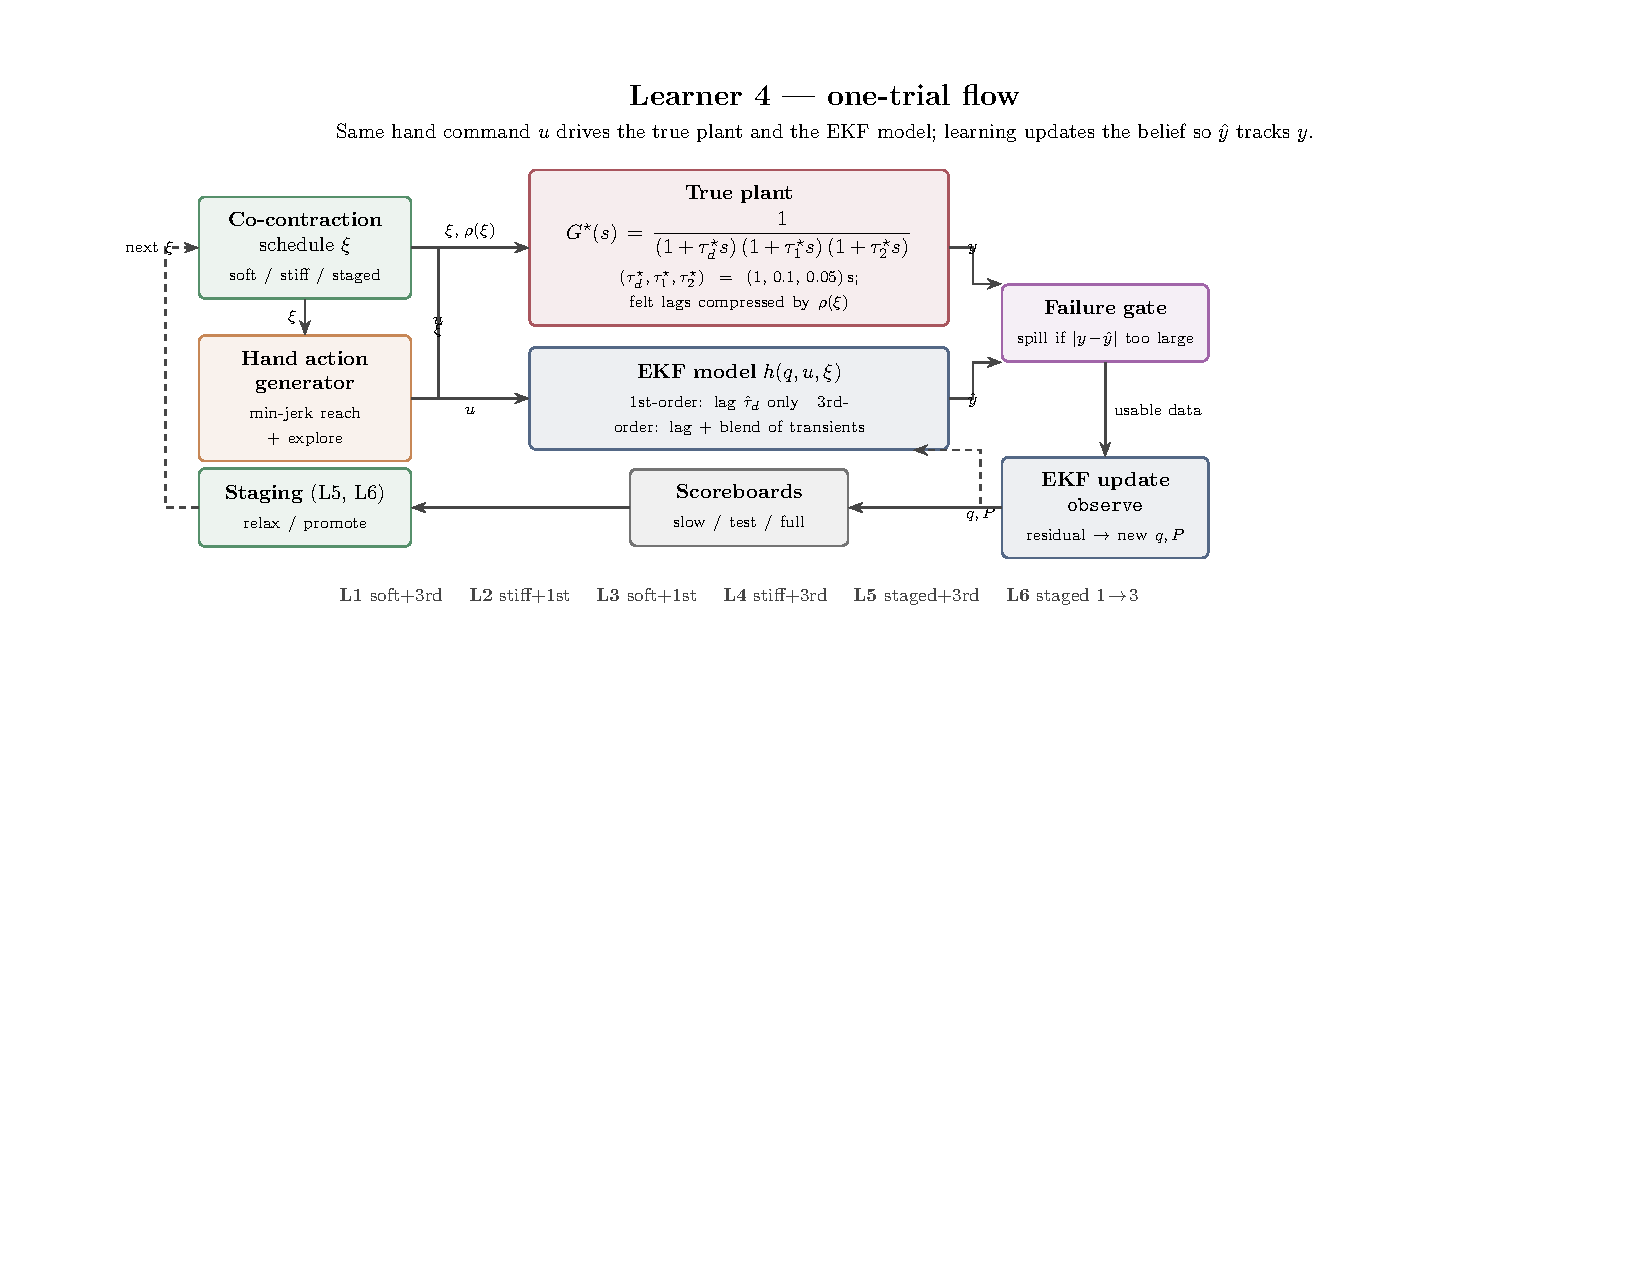
\includegraphics[width=\linewidth]{../outputs/learner4/learner4_block_diagram_simple.pdf}
\caption{Learner~4 one-trial flow (main blocks). Same hand command $u$
drives the true plant and the EKF model; the failure gate truncates bad
trials; \texttt{observe} updates the belief. A fuller annotated version is
\texttt{outputs/learner4/learner4\_block\_diagram.pdf}.}
\label{fig:learner4block}
\end{figure}

\subsubsection{The loop skeleton}

\begin{verbatim}
for n in range(n_trials):
    xi = _xi_for(condition, stage)
    ref = reach_reference(n_t, dt, t_move)
    u = ref + U_EXPLORE * band_limited_noise(...)
    y = cascade_exact(experienced_taus(TAU_TRUE, xi), u, dt) + noise
    y_hat = learner.predict(u, xi)
    # failure gate -> stop index
    if stop >= MIN_USABLE:
        learner.observe(u[:stop], y[:stop], xi)
    else:
        learner.drift()
    # log errors; maybe promote / relax stage
\end{verbatim}

Constants used below (Learner~4): $\dt=0.01$\,s, $T_{\mathrm{trial}}=2.5$\,s
so $n_t=250$, $t_{\mathrm{move}}=0.25$\,s (\texttt{FAST\_MOVE}),
\texttt{U\_EXPLORE}${}=0.10$, \texttt{NOISE\_STD}${}=0.012$,
\texttt{S\_BASE}${}=0.15$, \texttt{MIN\_USABLE}${}=20$.

% ----- step 1: xi -----------------------------------------------------------
\subsubsection{Step 1 --- grip $\xi$ for this condition}

\texttt{\_xi\_for(condition, stage)} returns:
\begin{itemize}[nosep]
\item soft schedule (L1, L3): $\xi=\xi_{\mathrm{soft}}=0.7$;
\item stiff schedule (L2, L4): $\xi=\xi_{\mathrm{stiff}}=3.0$;
\item staged (L5, L6): $\xi\in\{3.0,\,1.3,\,0.7\}$ according to stage.
\end{itemize}
Grip does \emph{not} change the true cup's $\tau^\star$; it changes the
\emph{felt} time constants via $\rho(\xi)$ (\S\ref{sec:rho},
\S\ref{sec:plant}).

% ----- step 2: ref ----------------------------------------------------------
\subsubsection{Step 2 --- planned reach \texttt{reach\_reference}}

\begin{verbatim}
ref = reach_reference(n_t, dt, t_move)
\end{verbatim}

This is \textbf{desired hand motion}, not the plant and not the felt signal.
Code (\texttt{plant.py}):

\begin{verbatim}
t = np.arange(n) * dt
out  = min_jerk(t, t_move)                          # forward
back = min_jerk(clip(t - (t_move+0.35), 0), t_move, amp=-1)
ref  = out + back
\end{verbatim}

\textbf{Minimum-jerk forward leg} (same as \eqref{eq:minjerk}):
\begin{equation}
s = \mathrm{clip}\!\Bigl(\frac{t}{t_{\mathrm{move}}},0,1\Bigr),\qquad
u_{\mathrm{out}}(t) = 10s^3 - 15s^4 + 6s^5.
\label{eq:l4minjerk}
\end{equation}
Then a mirrored return starting at $t=t_{\mathrm{move}}+0.35$:
\begin{equation}
u_{\mathrm{ref}}(t) = u_{\mathrm{out}}(t)
  - u_{\mathrm{out}}\bigl(\mathrm{clip}(t-(t_{\mathrm{move}}+0.35),0)\bigr).
\label{eq:l4ref}
\end{equation}

\begin{examplebox}{Why the first samples of \texttt{ref} are almost zero}
With $t_{\mathrm{move}}=0.25$\,s and $\dt=0.01$\,s the hand \emph{starts from
rest}.  The min-jerk polynomial begins as $\sim s^3$, so early position is tiny:

\begin{center}
\small
\begin{tabular}{@{}rrr@{}}
\toprule
$t$ (s) & $s=t/0.25$ & $u_{\mathrm{out}}$ (approx) \\
\midrule
$0.00$ & $0.00$ & $0.0000$ \\
$0.01$ & $0.04$ & $6.0\times10^{-4}$ \\
$0.02$ & $0.08$ & $4.5\times10^{-3}$ \\
$0.05$ & $0.20$ & $0.032$ \\
$0.25$ & $1.00$ & $1.000$ \\
\bottomrule
\end{tabular}
\end{center}

Then \texttt{ref} stays at $1$ during the pause ($0.25\to0.60$\,s), then the
return leg brings it back.  Those near-zero early samples are intentional
smooth acceleration, not a bug and not the third-order plant ``zeroing''
anything.
\end{examplebox}

% ----- step 3: u ------------------------------------------------------------
\subsubsection{Step 3 --- actual command $u$ (plan + exploration)}

\begin{verbatim}
u = ref + U_EXPLORE * band_limited_noise(n_t, dt, t_move, rng)
\end{verbatim}

\begin{equation}
u = u_{\mathrm{ref}} + 0.10\cdot u_{\mathrm{explore}},
\label{eq:l4u}
\end{equation}
where $u_{\mathrm{explore}}$ is unit-std band-limited noise
\eqref{eq:bandlimited}.  \texttt{rng} is a seeded random generator
(\texttt{np.random.default\_rng(seed)}) so each seed is reproducible but
every trial has a different wiggle.

\begin{examplebox}{Why band-limited, not white?}
White noise would jab every cup mode on every trial and make ``learn all
three modes from day one'' artificially easy.  Band-limited wiggles stay
inside what a smooth arm can produce; the only way to excite fast modes is
still to move \emph{fast} ($t_{\mathrm{move}}=0.25$\,s).  See
\S\ref{sec:plant}.
\end{examplebox}

% ----- step 4: plant y ------------------------------------------------------
\subsubsection{Step 4 --- true plant: $y$ from $u$}

\begin{verbatim}
y = cascade_exact(experienced_taus(TAU_TRUE, xi), u, dt)
    + NOISE_STD * rng.normal(size=n_t)
\end{verbatim}

\textbf{This is the third-order plant.}  $y$ is \emph{not} hand motion; it is
the \textbf{felt response} of the cup (and coupling) to hand motion $u$.

True object (fixed forever):
\begin{equation}
G^\star(s)=\frac{1}{(1+\tau_d^\star s)(1+\tau_1^\star s)(1+\tau_2^\star s)},
\qquad
(\tau_d^\star,\tau_1^\star,\tau_2^\star)=(1.0,\,0.1,\,0.05)\,\mathrm{s}.
\label{eq:l4true}
\end{equation}

\textbf{What grip changes} (\texttt{experienced\_taus}):
\begin{equation}
\rho(\xi)=\begin{cases}
1 & \xi\le 1,\\
\bigl(\xi+\sqrt{\xi^2-1}\bigr)^2 & \xi>1,
\end{cases}
\qquad
\tau_{\mathrm{felt}}=\Bigl(\tau_d^\star,\;
\tfrac{\tau_1^\star}{\rho(\xi)},\;
\tfrac{\tau_2^\star}{\rho(\xi)}\Bigr).
\label{eq:l4felt}
\end{equation}

\begin{examplebox}{Felt time constants at soft vs stiff}
Soft $\xi=0.7$: $\rho=1$, feel $(1.0,\,0.10,\,0.05)$ --- all three modes.\\
Stiff $\xi=3$: $\rho\approx34.3$, feel $(1.0,\,0.0029,\,0.0015)$ --- fast
modes settle in a few milliseconds; the cup \emph{feels} nearly first-order.
\end{examplebox}

\textbf{Cascade equations} (\texttt{cascade\_exact}): three first-order lags
in series.  Continuous intuition for one stage:
\begin{equation}
\tau\dot x = u_{\mathrm{in}}-x
\quad\Leftrightarrow\quad
\frac{X(s)}{U_{\mathrm{in}}(s)}=\frac{1}{1+\tau s}.
\end{equation}
Discrete update used in code (\eqref{eq:lagdisc}):
\begin{equation}
a=e^{-\dt/\tau},\qquad
x[k]=a\,x[k-1]+(1-a)\,u_{\mathrm{in}}[k].
\label{eq:l4lag}
\end{equation}
Chained:
\begin{align}
z^{(1)} &= \mathrm{Lag}(\tau_d^\star)\,[u], \nonumber\\
z^{(2)} &= \mathrm{Lag}(\tau_1^\star/\rho)\,[z^{(1)}], \nonumber\\
y_{\mathrm{plant}} &= \mathrm{Lag}(\tau_2^\star/\rho)\,[z^{(2)}],
\label{eq:l4cascade}
\end{align}
then sensor noise:
\begin{equation}
y = y_{\mathrm{plant}} + 0.012\,\varepsilon,
\qquad \varepsilon\sim\mathcal N(0,I_{n_t}).
\label{eq:l4y}
\end{equation}

\begin{examplebox}{Numeric lag step}
$\dt=0.01$, $\tau=1.0$: $a=e^{-0.01}\approx0.990$.  Each sample keeps 99\%
of the previous felt value and admits 1\% of the new input --- a slow
memory.  For a compressed fast mode $\tau=0.0029$: $a=e^{-0.01/0.0029}\approx0.032$,
almost a pass-through (``already settled'').
\end{examplebox}

% ----- step 5: predict ------------------------------------------------------
\subsubsection{Step 5 --- brain prediction $\hat y=\texttt{learner.predict}(u,\xi)$}

\begin{verbatim}
y_hat = learner.predict(u, xi)   # -> _h(self.q, u, xi)
\end{verbatim}

Same $u$ and $\xi$, but through the \textbf{learner's adjustable copy} of the
cup, not through $\tau^\star$.

\textbf{Full learner} (\texttt{TwoTimescaleEKF}; L1, L4, L5, L6 after promote).
Belief state:
\begin{equation}
q=\bigl[\log\hat\tau_d,\;\log\hat\tau_1,\;\log\hat\tau_2,\;w_1,\;w_2\bigr]^\top.
\label{eq:l4q}
\end{equation}
Prediction chain (\S\ref{sec:learner2}; code \texttt{\_h}):
\begin{align}
x^{(0)} &= u, \nonumber\\
x^{(1)} &= \mathrm{Lag}(\hat\tau_d)\,[x^{(0)}], \nonumber\\
x^{(2)} &= \mathrm{Blend}\bigl(\hat\tau_1/\rho(\xi),\,w_1\bigr)\,[x^{(1)}], \nonumber\\
\hat y &= \mathrm{Blend}\bigl(\hat\tau_2/\rho(\xi),\,w_2\bigr)\,[x^{(2)}],
\label{eq:l4h}
\end{align}
with blend
\begin{equation}
\mathrm{Blend}(\tau,w)[x]=(1-w)\,x + w\cdot\mathrm{Lag}(\tau)[x]
\label{eq:l4blend}
\end{equation}
(\S\ref{sec:learner2}: $w$ turns a fast mode on/off \emph{without} killing
$\tau\to0$, so pruning stays reversible).  Effective order:
\begin{equation}
\neff = 1 + w_1 + w_2.
\label{eq:l4neff}
\end{equation}

\textbf{Slow-only learner} (\texttt{FirstOrderEKF}; L2, L3, early L6):
\begin{equation}
\hat y = \mathrm{Lag}(\hat\tau_d)\,[u]
\qquad\text{($q=[\log\hat\tau_d]$ only; $\xi$ unused in $h$).}
\label{eq:l4h1}
\end{equation}

\begin{examplebox}{Plant vs $h$ --- same family, not the same cup}
\begin{center}
\small
\begin{tabular}{@{}lll@{}}
\toprule
 & True plant $y$ & Belief $h\to\hat y$ \\
\midrule
Time constants & fixed $\tau^\star$ & learned from $q$ \\
Fast modes & always full lags & blended by $w_1,w_2$ \\
Noise & yes ($0.012$) & clean prediction \\
\bottomrule
\end{tabular}
\end{center}
When $w_1=w_2=1$ and $\hat\tau\approx\tau^\star$, $\hat y\approx y_{\mathrm{plant}}$.
Early trials they do not match --- that mismatch is what drives learning.
\end{examplebox}

% ----- step 6: failure ------------------------------------------------------
\subsubsection{Step 6 --- spill / failure gate}

\begin{verbatim}
tolerance = S_BASE * xi / XI_SOFT
over = np.flatnonzero(np.abs(y - y_hat) > tolerance)
failed = over.size > 0
stop = int(over[0]) if failed else n_t
\end{verbatim}

\begin{equation}
\text{tolerance} = 0.15\cdot\frac{\xi}{0.7},
\qquad
\text{fail if } |y[k]-\hat y[k]| > \text{tolerance for some }k.
\label{eq:l4fail}
\end{equation}
\textbf{Layman:} if prediction is too far from feel, you ``spill'' and the
trial stops at the first bad sample.  Stiffer grip raises tolerance
(more room for error while braced).  Only the prefix $u[:\texttt{stop}]$,
$y[:\texttt{stop}]$ is available to learn from.

% ----- step 7: observe ------------------------------------------------------
\subsubsection{Step 7 --- \texttt{observe}: the EKF learns (or \texttt{drift})}

\begin{verbatim}
if stop >= MIN_USABLE:          # need >= 20 samples
    stats = learner.observe(u[:stop], y[:stop], xi)
else:
    learner.drift()             # P <- P+Q; q unchanged
\end{verbatim}

\texttt{observe} is where the Extended Kalman Filter updates beliefs
(\S\ref{sec:ekf}).  \texttt{predict} only \emph{uses} $q$; \texttt{observe}
\emph{changes} $q$ and $P$.

\paragraph{Layman story.}
You felt $y$, expected $\hat y=h(q,u,\xi)$, saw residual $e=y-\hat y$.
\texttt{observe} asks: ``which knobs in $q$ would shrink that residual, and how
sure am I?'' then nudges those knobs a little.

\paragraph{Equations (full \texttt{TwoTimescaleEKF.observe}).}

Prior / process:
\begin{equation}
q^- = q,\qquad P^- = P+Q,\qquad P_{\mathrm{inv}}=(P^-)^{-1}.
\label{eq:l4prior}
\end{equation}

Iterate $m=1,\ldots,3$ (\texttt{IEKF\_ITERS}; re-linearise each time):
\begin{align}
\hat y &= h(q,u,\xi), \label{eq:l4obs1}\\
e &= (y-\hat y)_{\downarrow\mathrm{THIN}}, \label{eq:l4obs2}\\
H_{:,i} &= \frac{h(q+\varepsilon e_i)-h(q)}{\varepsilon}
  \quad\text{(finite-diff.\ Jacobian; then thin)}, \label{eq:l4obs3}\\
R &= \max\bigl(\sigma_R^2,\;\overline{e^2}\bigr), \label{eq:l4obs4}\\
A &= P_{\mathrm{inv}} + \frac{H^\top H}{R} + \diag(\alpha), \label{eq:l4obs5}\\
P^+ &= A^{-1}, \label{eq:l4obs6}\\
\Delta q &= P^+\Biggl(
  \underbrace{\frac{H^\top e}{R}}_{\text{data pull}}
  -\underbrace{\alpha(q-q_{\mathrm{target}})}_{\text{ARD: pull }w\to0}
  -\underbrace{P_{\mathrm{inv}}(q-q^-)}_{\text{stay near prior}}
\Biggr), \label{eq:l4obs7}\\
q &\leftarrow \mathrm{clip}\bigl(q+\mathrm{clip}(\Delta q,\pm\Delta_{\max}),\,q_{\mathrm{lo}},q_{\mathrm{hi}}\bigr).
\label{eq:l4obs8}
\end{align}
Commit $q\leftarrow q$, $P\leftarrow P^++\varepsilon I$.  Then ARD refreshes
$\alpha$ on $w_1,w_2$ only (\S\ref{sec:ekf}).

\begin{stepbox}{What each line means in plain English}
\begin{enumerate}[nosep]
\item \eqref{eq:l4obs1}--\eqref{eq:l4obs2}: recompute expected feel and the
  surprise $e$.
\item \eqref{eq:l4obs3}: for each knob, ``if I tweak you, how does $\hat y$
  change?''
\item \eqref{eq:l4obs4}: early big errors are model error, not tiny sensor
  noise --- do not become overconfident too soon.
\item \eqref{eq:l4obs5}--\eqref{eq:l4obs7}: information-form Kalman update
  plus a prior that prefers small fast-mode weights unless the data clearly
  need them.
\item \eqref{eq:l4obs8}: take a bounded step so one messy trial cannot wreck
  the model.
\end{enumerate}
\end{stepbox}

\begin{examplebox}{Tiny numeric intuition for one update}
Suppose truth $\tau_d^\star=1.0$ but belief $\hat\tau_d=0.30$.  Then $h$
responds too fast; $e$ has a clear pattern; the $\log\hat\tau_d$ column of $H$
says ``increasing $\hat\tau_d$ would help''; $\Delta q$ bumps $\log\hat\tau_d$
up a little.  After many trials $\hat\tau_d\to1$, $e$ shrinks, and the
diagonal of $P$ for that entry gets smaller (more confident).  Under stiff
$\xi$, $e$ barely depends on $w_1,w_2$, so ARD shrinks them and
$\neff\to1$.
\end{examplebox}

\texttt{FirstOrderEKF.observe} is the same loop with
$q=[\log\hat\tau_d]$ only and no ARD term.

% ----- step 8: score / stage ------------------------------------------------
\subsubsection{Step 8 --- scoreboards, TTC, and staging / promote}

After the update, every trial logs three errors (and friends):
\begin{align}
\texttt{bias\_d} &= \hat\tau_d - \tau_d^\star, \nonumber\\
\texttt{err} &= \text{full-object impulse relative error}, \nonumber\\
\texttt{test\_err} &= \text{relative error on the common soft fast probe}.
\label{eq:l4scores}
\end{align}

\textbf{Common test probe} (built once per seed; identical for every L):
\begin{verbatim}
probe_u = reach_reference(...)           # clean ref, no exploration
probe_y = cascade_exact(felt at XI_SOFT, probe_u)
test_err = ||probe_y - learner.predict(probe_u, XI_SOFT)|| / ||probe_y||
\end{verbatim}
So the fair exam is always: \emph{``Can you predict a soft, fast reach?''}
even if you trained while stiff.

Time-to-criterion requires the relevant error below threshold for
\texttt{CRITERION\_STREAK}${}=3$ consecutive trials
(\texttt{SLOW\_CRITERION}${}=0.08$, \texttt{FULL}/\texttt{TEST}${}=0.10$).

\textbf{Staged L5/L6.}  After enough trials in a stage and
$\mathrm{sd}(\log\hat\tau_d)<0.04$, stage advances
$\xi:3.0\to1.3\to0.7$.  On L6's first advance, \texttt{\_promote} copies
only $\log\hat\tau_d$ and its variance into a fresh \texttt{TwoTimescaleEKF};
$w_1,w_2,\hat\tau_1,\hat\tau_2$ start from the usual prior.

% ----- big picture ----------------------------------------------------------
\subsubsection{Putting the whole chain together}

\begin{equation}
\boxed{\;
\begin{aligned}
&u_{\mathrm{ref}}\xrightarrow{\;+\,0.1\,u_{\mathrm{explore}}\;} u \\
&u \xrightarrow{\;\text{true cascade at }\tau_{\mathrm{felt}}(\xi)\;}
  y_{\mathrm{plant}}\xrightarrow{\;+\,\text{noise}\;} y \\
&u \xrightarrow{\;h(q,\xi)\;} \hat y \\
&e=y-\hat y \xrightarrow{\;\texttt{observe}\;} q^+,\,P^+
\end{aligned}
\;}
\label{eq:l4pipeline}
\end{equation}

\begin{resultbox}{What this loop is testing}
Same plant, same fast reach, six learning policies (L1--L6).  The question is
not ``can an EKF fit a known model?'' --- it is whether \textbf{co-contracting
so that the world looks first-order} lets a person (or agent) learn the slow
part safely and then, by relaxing / promoting, acquire the full soft-cup
behaviour on the shared test probe.
\end{resultbox}

\subsection{Three scoreboards}

\begin{center}
\small
\begin{tabular}{@{}lll@{}}
\toprule
Name & Measure & Criterion \\
\midrule
slow & $|\hat\tau_d-\tau_d|$, the part a person keeps & $<0.08$\,s \\
full & impulse error of the belief about the whole object & $<0.10$ \\
test & relative error predicting a common soft, fast probe & $<0.10$ \\
\bottomrule
\end{tabular}
\end{center}

The \textbf{test} scoreboard is the fair one. Every condition is asked to
predict the same deterministic, noise-free soft reach, whatever stiffness it
happens to be holding, so ``I can only do this while braced'' appears as a
cost instead of being hidden. The slow criterion is tighter than the soft
first-order bias floor $(\tau_1+\tau_2)/\rho(0.7)=0.150$\,s, so L3 cannot
reach it unless the bias law \eqref{eq:bias_law} is wrong.

\begin{figure}[ht]
\centering
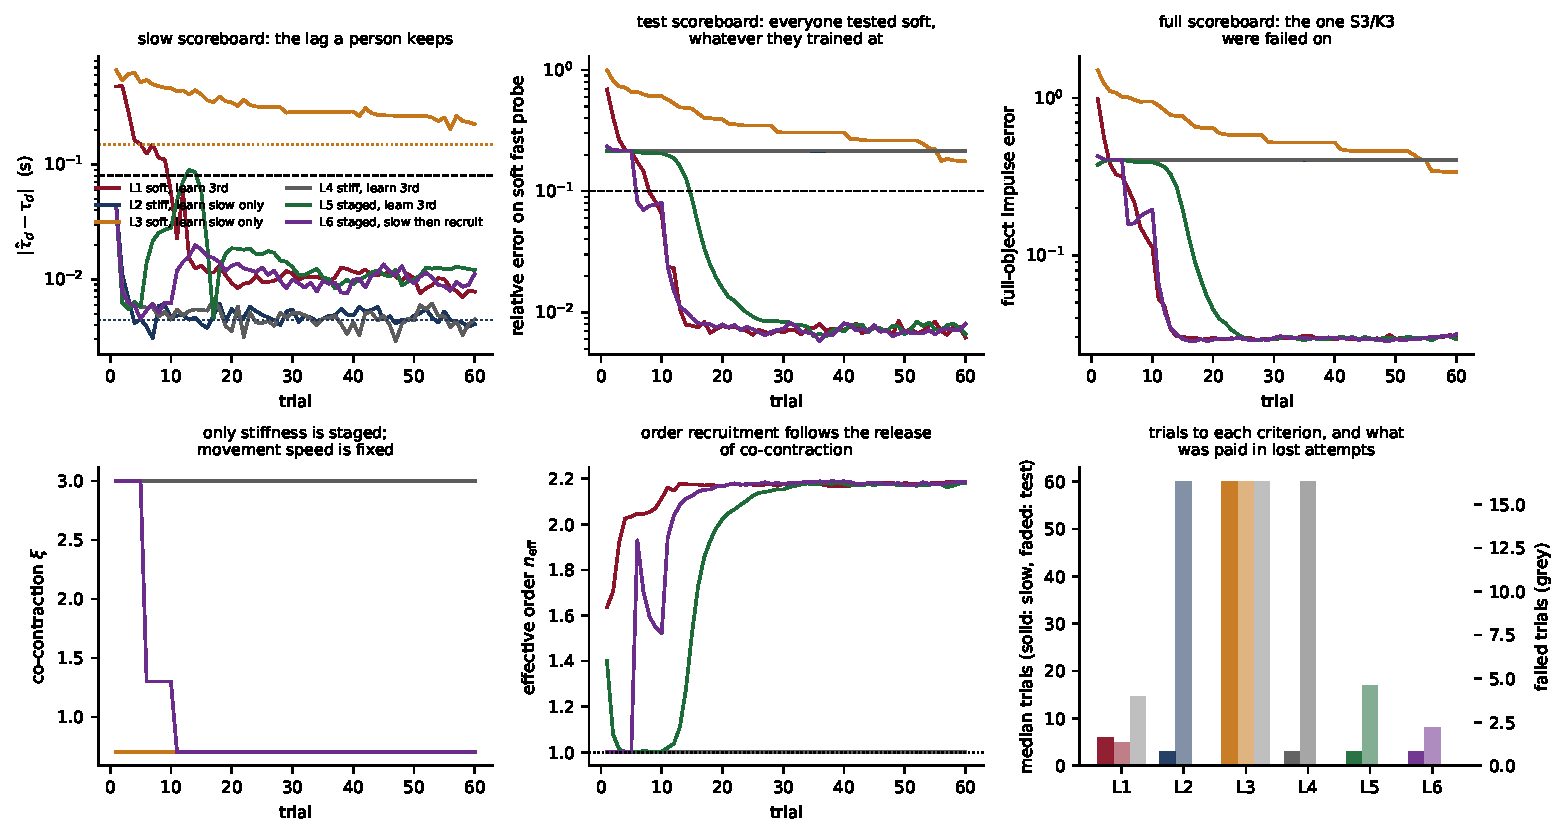
\includegraphics[width=\linewidth]{../outputs/learner4/learner4.pdf}
\caption{Learner~4, 20 seeds, 60 trials. Top row, the three scoreboards:
error in the dominant lag, error on the common soft probe, and full-object
impulse error. Bottom row: the stiffness schedule (movement speed is fixed
throughout), emergent effective order, and trials to criterion against
failed attempts. Every co-contracting strategy reaches the slow lag in three
trials; only the ones that eventually relax reach the soft probe at all.}
\label{fig:learner4}
\end{figure}

\begin{resultbox}{Co-contraction halves the trials to the slow lag (20 seeds, 60 trials)}
\begin{center}
\small
\begin{tabular}{@{}lrrrrrrr@{}}
\toprule
 & slow & test & full & peak $|\Delta\tau_d|$ & test err & $\neff$ & failed \\
\midrule
L1 soft, 3rd          & 6     & \textbf{5} & \textbf{5} & $0.691$\,s & $0.007$ & $2.18$ & $4.0$ \\
L2 stiff, slow-only   & \textbf{3} & never & never & $0.015$\,s & $0.216$ & $1.00$ & $0.0$ \\
L3 soft, slow-only    & never & never & never & $0.962$\,s & $0.175$ & $1.00$ & $16.3$ \\
L4 stiff, 3rd         & \textbf{3} & never & never & $0.015$\,s & $0.215$ & $1.00$ & $0.0$ \\
L5 staged, 3rd        & \textbf{3} & 17 & 19 & $0.092$\,s & $0.007$ & $2.18$ & $0.0$ \\
L6 staged, warm-start & \textbf{3} & 8 & 13 & $0.025$\,s & $0.007$ & $2.19$ & $0.0$ \\
\bottomrule
\end{tabular}
\end{center}

Holm-corrected two-sided Mann--Whitney. On the slow scoreboard: L2, L5 and
L6 each beat L1 by $-3$ trials, $p=3.9\times10^{-7}$; L2 vs L4 is a tie;
L2 beats L3 by $-58$, $p=3.8\times10^{-9}$. On the test scoreboard: L5 is
\emph{slower} than L1 by $+12$, $p=3.7\times10^{-8}$, and L6 beats L5 by
$-9$, $p=1.8\times10^{-8}$.
\end{resultbox}

\subsection{Ranking the conditions: best to worst}
\label{sec:learner4rankings}

The ``best'' condition depends entirely on which scoreboard you care about.
There is no single winner across all three rulers; that is the point of
Learner~4.  Table~\ref{tab:learner4rankings} lists the median ordering on
each scoreboard (20 seeds, 60 trials).  ``never'' means the condition did
not reach the criterion within 60 trials.

\small
\begin{longtable}{@{}p{2.6cm}p{5.8cm}p{5.8cm}@{}}
\caption{Best-to-worst ordering for each scoreboard and safety measure.
Ties share a rank.  Read down each column: first row is best, last is worst.}
\label{tab:learner4rankings}\\
\toprule
\textbf{Scoreboard / measure} & \textbf{Best $\to$ worst (median trials or value)} &
\textbf{Plain-language reading} \\
\midrule
\endfirsthead
\toprule
\textbf{Scoreboard / measure} & \textbf{Best $\to$ worst} &
\textbf{Plain-language reading} \\
\midrule
\endhead
Slow lag
($|\hat\tau_d-\tau_d|<0.08$\,s) &
\makecell[l]{%
\textbf{1st (tie):} L2, L4, L5, L6 --- 3 trials\\[2pt]
\textbf{2nd:} L1 --- 6 trials\\[2pt]
\textbf{Worst:} L3 --- never} &
Co-contraction halves the trials to learn the sluggishness everyone keeps.
L3 fails because there is no filter. \\
\addlinespace
Soft test
(common unbraced reach; failures free) &
\makecell[l]{%
\textbf{1st:} L1 --- 5 trials\\[2pt]
\textbf{2nd:} L6 --- 8 trials\\[2pt]
\textbf{3rd:} L5 --- 17 trials\\[2pt]
\textbf{Worst (tie):} L2, L3, L4 --- never} &
If spilling costs nothing, going soft immediately wins the fair exam.
Staying stiff forever (L2, L4) never passes; staging (L5, L6) eventually
does, but slower than L1. \\
\addlinespace
Full object
(impulse error $<0.10$; failures free) &
\makecell[l]{%
\textbf{1st:} L1 --- 5 trials\\[2pt]
\textbf{2nd:} L6 --- 13 trials\\[2pt]
\textbf{3rd:} L5 --- 19 trials\\[2pt]
\textbf{Worst (tie):} L2, L3, L4 --- never} &
Same story as the soft test: the deep end is fastest on the old Learner~2
ruler when failures are free. \\
\addlinespace
Failed trials
(lower is better) &
\makecell[l]{%
\textbf{Best (tie):} L2, L4, L5, L6 --- 0.0\\[2pt]
\textbf{2nd:} L1 --- 4.0\\[2pt]
\textbf{Worst:} L3 --- 16.3} &
Every co-contracting strategy is perfectly safe.  L1 spills occasionally.
L3 is catastrophic: wrong model \emph{and} constant spills. \\
\addlinespace
Peak error in slow lag
(lower is better) &
\makecell[l]{%
\textbf{Best (tie):} L2, L4 --- 0.015\,s\\[2pt]
\textbf{2nd:} L6 --- 0.025\,s\\[2pt]
\textbf{3rd:} L5 --- 0.092\,s\\[2pt]
\textbf{4th:} L1 --- 0.691\,s\\[2pt]
\textbf{Worst:} L3 --- 0.962\,s} &
How wrong you were about sluggishness at your \emph{worst} moment along the
learning curve.  Co-contraction keeps that swing small; the deep end and
L3 swing wildly. \\
\addlinespace
Effective trials to soft test
when each failure costs $k$ extra trials &
\makecell[l]{%
$k=0$: L1 (5) $<$ L6 (8) $<$ L5 (17)\\[2pt]
$k=1$: L6 (8) $=$ L1 (8) $<$ L5 (17)\\[2pt]
$k\ge2$: L6 (8) $<$ L5 (17) $<$ L1 (11+)\\[2pt]
$k=5$: L6 (8) $<$ L5 (17) $<$ L1 (20)\\[2pt]
\textbf{Never competitive:} L2, L3, L4} &
Once recovering from a spill costs even \emph{one} extra trial, warm-started
staging (L6) draws level with or beats the deep end.  L2 and L4 never learn
the unbraced reach at all. \\
\bottomrule
\end{longtable}
\normalsize

\begin{resultbox}{Overall verdict by goal}
\begin{itemize}[nosep]
\item \textbf{Goal: learn the slow lag quickly and safely.}\;
  Best: \textbf{L2 = L4 = L5 = L6} (3 trials, 0 failures).\;
  Worst: \textbf{L3} (never; 16 failures).
\item \textbf{Goal: learn the whole cup fastest, spills are free.}\;
  Best: \textbf{L1} (5 trials).\;
  Worst: \textbf{L2, L3, L4} (never on the soft test).
\item \textbf{Goal: learn the whole cup fastest, spills cost anything.}\;
  Best: \textbf{L6} (8 effective trials from $k=1$ upward).\;
  Second: \textbf{L5} (17 trials, overtakes L1 at $k=5$).\;
  Worst on safety \emph{and} speed: \textbf{L3}.
\item \textbf{Goal: understand the mechanism.}\;
  L4 ties L2 on slow lag $\Rightarrow$ the \emph{filter} does the work, not
  restricting to one parameter.\;
  L3 fails $\Rightarrow$ you cannot treat transients as noise without
  co-contraction first.
\end{itemize}
\end{resultbox}

\begin{examplebox}{One-sentence character sketch of each condition}
\textbf{L1} --- fast and reckless learner;\;
\textbf{L2} --- safe slow learner who never finishes the textbook;\;
\textbf{L3} --- worst of both worlds (wrong and unsafe);\;
\textbf{L4} --- proves the plant filters itself while stiff;\;
\textbf{L5} --- Thrish's patient curriculum (safe, complete, slow if spills
are free);\;
\textbf{L6} --- L5 done properly: the slow chapter is \emph{transferred}, not
re-learned.
\end{examplebox}

\subsection{What the comparison shows}

\begin{enumerate}[nosep]
\item \textbf{Co-contraction does learn the slow dynamics faster.} Three
  trials against six, with zero failed attempts against four. Every
  co-contracting strategy shows it. This is the claim, and it holds.
\item \textbf{The filter does the work, not the restriction.} L2 and L4 are
  an exact tie. Once co-contraction has compressed the transients, a full
  third-order EKF prunes itself to $\neff=1.00$ and learns $\tau_d$ just as
  fast as a learner that was never offered the extra modes. Order reduction
  is a property of the coupled plant, not a modelling choice.
\item \textbf{Neglecting the transients is only legitimate after the
  filter.} L3 never reaches criterion, plateaus at $+0.218$\,s of bias, and
  loses $16$ trials. Calling the transients ``noise'' is correct once
  $\rho(\xi)$ has removed them and a systematic error before that.
\item \textbf{On the whole object, staging is still not a shortcut.}
  Tested on the common soft probe, L1 arrives in 5 trials, L6 in 8, L5 in
  17. The staged learner spends its first $\sim$15 trials in a regime where
  the transients are not in the data at all, so it cannot learn them however
  good its slow model becomes. L2, which never relaxes, never arrives.
\item \textbf{Warm-starting recovers most of that loss.} L6 beats L5 by 9
  trials purely by handing the converged slow lag across. If a curriculum is
  to be defended, the value is in the \emph{transfer} of the slow estimate,
  not in the staging.
\end{enumerate}

\subsection{The failure cost decides the full-model comparison}
\label{sec:failurecost}

The simulation charges nothing for a failed attempt beyond losing the rest
of that trial's data, which is the most generous possible assumption for a
learner that goes straight to the deep end. Charging a recovery overhead of
$k$ extra trials per failure --- the sweep this report previously
pre-registered as the way the ordering might flip --- gives the effective
trials to the soft-probe criterion:

\begin{center}
\small
\begin{tabular}{@{}lrrrrrrrr@{}}
\toprule
recovery cost $k$ & $0$ & $0.5$ & $1$ & $2$ & $3$ & $5$ & $8$ & $12$ \\
\midrule
L1 soft              & $5.0$ & $6.5$ & $8.0$ & $11.0$ & $14.0$ & $20.0$ & $29.0$ & $41.0$ \\
L5 staged            & $17.0$ & $17.0$ & $17.0$ & $17.0$ & $17.0$ & $17.0$ & $17.0$ & $17.0$ \\
L6 staged, warm-start & $8.0$ & $8.0$ & $8.0$ & $8.0$ & $8.0$ & $8.0$ & $8.0$ & $8.0$ \\
\bottomrule
\end{tabular}
\end{center}

\begin{figure}[ht]
\centering
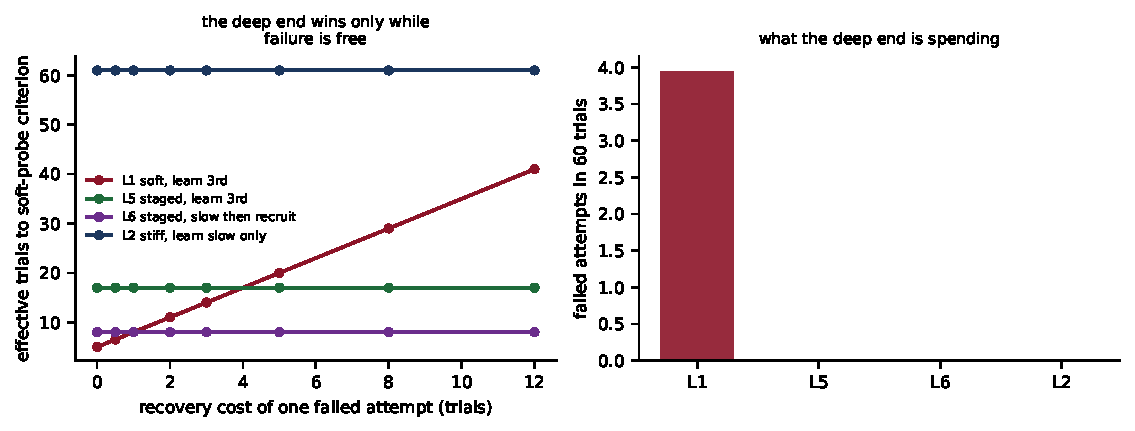
\includegraphics[width=0.86\linewidth]{../outputs/learner4/failure_cost.pdf}
\caption{The staged learners are flat because they never fail. L6 draws
level with the deep end as soon as one failed attempt costs a single extra
trial and wins outright beyond that; L5 overtakes at a cost of five.}
\label{fig:failurecost}
\end{figure}

So the full-model claim is conditional, and the condition is cheap to
satisfy: \emph{if recovering from a dropped attempt costs anything at all,
co-contracting to learn is also the faster route to the whole model.} For a
cup of coffee, a bicycle or a trainee surgeon, a failed attempt costs a
great deal more than one trial.

\begin{warnbox}{Do not claim these}
\begin{itemize}[nosep]
\item ``Restricting the learner to first order is what speeds learning.''
  L4 refutes it: a full-order learner held stiff is exactly as fast.
\item ``Staging is faster than the deep end, full stop.'' With free
  failures it is 12--14 trials \emph{slower}. The claim requires a non-zero
  failure cost, which should be stated rather than assumed.
\item ``A learner that stays stiff eventually learns the object.'' L2 never
  reaches the soft-probe criterion and plateaus at a test error of $0.216$.
  Co-contraction buys a correct slow model; only relaxation buys the
  transients.
\end{itemize}
\end{warnbox}

\begin{warnbox}{Parameter sensitivity}
The 12-trial staging penalty in L5 is set by the forced dwell
(\texttt{MIN\_TRIALS\_PER\_STAGE} $=5$ across three stages), not by the
physics. The break-even failure costs in \S\ref{sec:failurecost} move with
it, so quote them as order-of-magnitude rather than to two significant
figures.
\end{warnbox}

% =============================================================================
\section{Part IX --- Conclusions and discussion}
\label{sec:conclusions}
% =============================================================================

\subsection{What we conclude}

\begin{enumerate}
\item \textbf{Co-contraction manufactures time-scale separation} through the
  exact closed form $\rho(\xi)=(\xi+\sqrt{\xi^2-1})^2$ \eqref{eq:rho}, derived
  directly from the mass--spring--damper physics \eqref{eq:msd}--\eqref{eq:reduced}.
  This part of the mechanism is uncontroversial physics, not a modelling
  choice, and both learners implement it identically.

\item \textbf{The precise, provable benefit for a low-order learner is bias
  reduction} \eqref{eq:bias_law}, not the generic ``fewer parameters therefore
  fewer trials needed'' argument originally proposed. Stiffening divides the
  \emph{misspecification bias} of a reduced-order fit by $\rho(\xi)$. This is
  a statement about a \emph{systematic} error, not a random one, so unlike
  the sample-complexity argument it does not require appealing to how a
  learner's optimisation algorithm behaves --- it is true of the
  \emph{best possible} low-order fit, and it is measurable directly in
  people by relating a participant's fitted dominant time constant to their
  measured EMG co-contraction level.

\item \textbf{Progressive order recruitment can emerge from data alone}
  (Learner~2, condition K2): $\neff$ holds at almost exactly 1 while stiff and
  rises to about 2.2 precisely when co-contraction is relaxed, with no rule
  in the code ever specifying how many modes to use at a given time --- it is
  a consequence of the ARD mechanism (\S\ref{sec:ard}) responding to which
  directions the data currently support.

\item \textbf{Staying stiff forever leaves a learner provably stuck at first
  order} (condition K3): $\neff$ settles at exactly $1.00$, the dominant
  estimate $\hat\tau_d$ is essentially unbiased (error $+0.0014$\,s), and the
  overall model error plateaus around $0.40$ and never improves. This is
  discovered by the learner, not imposed by the code, which is the crucial
  methodological improvement over Learner~1's version of the same claim.

\item \textbf{The curriculum reduces risk, not trial count}, in every
  simulation run of Learners~1--3: S2 and K2 both have zero failed trials
  against 10--12 for the corresponding deep-end schedules S1/K1, while taking
  \emph{more} trials, not fewer, to reach the same full-object model quality.

\item \textbf{Scoring the slow lag, which is what a person keeps, does
  produce a speed result} (Learner~4, \S\ref{sec:learner4}). Every
  co-contracting strategy reaches $|\hat\tau_d-\tau_d|<0.08$ in a median of
  3 trials against 6 for a soft third-order learner
  ($p=3.9\times10^{-7}$), with zero failed trials against four. The same
  first-order learner without the filter never arrives. The speed-up is
  manufactured by the plant becoming first-order, not by restricting the
  estimator: the stiff third-order cell is a tie with the stiff first-order
  cell.

\item \textbf{On the whole object the advantage is conditional on the cost
  of a failed attempt}, and that condition is now quantified rather than
  speculated about (\S\ref{sec:failurecost}). With failures free, staging
  costs 12--14 trials. Charging a recovery overhead of even one trial per
  failure brings the warm-started staged learner level with the deep end,
  and beyond that it wins, because it never fails at all. The earlier
  ``curriculum is safer, not faster'' conclusion was therefore an artefact
  of pricing failure at zero.

\item \textbf{A person starting stiff and relaxing later is rational} if their
  objective is something like ``do not lose attempts to catastrophic failure
  while building a coarse but useful model of a new object'', rather than
  ``minimise the number of attempts needed to fully identify a correctly
  specified model as fast as statistically possible''. The two objectives
  favour opposite strategies in these simulations, and the second objective
  is not, on reflection, a plausible description of how a person actually
  learns to handle a new object.
\end{enumerate}

\subsection{What we do \emph{not} conclude}

\begin{warnbox}{Do not claim these in the proposal --- both simulations refute them}
\begin{itemize}[nosep]
\item ``S2/K2 reaches criterion in fewer trials than S1/K1'' --- \textbf{false}
  in both learners, on every metric reported here. If anything the opposite is
  true.
\item ``The sample-complexity inequality $N(r,\delta)\propto\sigma^2r/(\delta\lambda_{\min}(\Phi_r))$ implies
  faster behavioural learning under a curriculum'' --- refuted specifically
  for Learner~1 by the diagnostic in \S\ref{sec:diag}: ill-conditioned
  parameter directions are also behaviourally cheap directions, so a bound on
  parameter error is not a bound on behavioural error.
\item ``Bandwidth staging alone (condition K4, speed changes without any
  stiffness change) is worse than the full stiffness-plus-speed curriculum
  (K2)'' --- in Learner~2, K4 is in fact among the \emph{fastest} schedules,
  reaching criterion in a median of only 4 trials.
\item ``A learner will always eventually recruit all three true modes''
  --- $\neff$ asymptotes near 2.2, not 3, in every condition that reaches a
  final answer, because under the band-limited exploration actually used
  (\eqref{eq:bandlimited}), the third (fastest) mode very rarely produces
  enough signal to be worth keeping according to the ARD criterion. This is
  the ARD mechanism working correctly, not a bug.
\end{itemize}
\end{warnbox}

\subsection{Recommended claim for the URF four-pager}

\begin{quote}
\emph{A learner that treats the coupled hand-object system as lower order than
it truly is inherits a systematic bias set by the neglected transient modes.
Co-contraction divides that bias by the exact separation ratio $\rho(\xi)$
derived from the coupled mass-spring-damper dynamics, yielding an unbiased
estimate of the dominant mode while the effective order of the internal model
is temporarily suppressed. A learner that carries its own uncertainty over how
many modes are currently supported by the data exhibits progressive order
recruitment exactly when co-contraction is relaxed, reaching the same
asymptotic model of the object as an unstiffened learner, but with
substantially lower peak error in the dominant mode along the way and no
failed attempts.}
\end{quote}

\subsection{Open next steps (not yet simulated)}

\begin{itemize}[nosep]
\item \textbf{Close the loop.} Both learners identify a plant; neither
  controls one. A controller designed from the current posterior belief,
  with co-contraction setting its gain margin, is the natural next condition,
  and it would let instability during learning enter as part of the
  phenomenon being studied rather than being engineered away.
\item \textbf{Sweep the cost of a failed trial.} \emph{Done} ---
  \S\ref{sec:failurecost}. The ordering does reverse, and it reverses at a
  recovery cost of about one trial for the warm-started staged learner.
  What remains open is calibrating that cost against a real task rather
  than sweeping it.
\item \textbf{Test the bias law directly against WP1 data.} Fit each
  participant's behaviour with a deliberately reduced-order model and check
  whether the residual bias in their fitted dominant time constant tracks
  $1/\rho(\hat\xi)$ computed from their own measured electromyographic
  co-contraction.
\end{itemize}

% =============================================================================
\section{Appendix --- Code map}
\label{sec:code}
% =============================================================================

\begin{center}
\small
\begin{tabular}{@{}ll@{}}
\toprule
\textbf{File} & \textbf{Role} \\
\midrule
\texttt{order\_reduction/plant.py} & Object \eqref{eq:thirdorder}, $\rho(\xi)$ \eqref{eq:rho}, cascades \eqref{eq:lagdisc}, reach \eqref{eq:minjerk}, exploration \eqref{eq:bandlimited} \\
\texttt{order\_reduction/learner.py} & Learner~1: gradient descent \eqref{eq:gd} \\
\texttt{order\_reduction/experiment.py} & S1--S5 trial loop, failure rule \eqref{eq:surprise}--\eqref{eq:tolerance} \\
\texttt{order\_reduction/diagnose.py} & $\kappa(\Phi)$ \eqref{eq:kappa} and behavioural cost \\
\texttt{order\_reduction/bias.py} & Bias law \eqref{eq:bias_law} verification \\
\texttt{order\_reduction/kalman\_learner.py} & Learner~2 / L1,L4,L5,L6 EKF: $h$, blend, \texttt{observe} \eqref{eq:l4h}--\eqref{eq:l4obs8}; ARD \eqref{eq:ard} \\
\texttt{order\_reduction/experiment2.py} & K1--K5 trial loop \\
\texttt{order\_reduction/slow\_learner.py} & First-order EKF on $\log\tau_d$ only \eqref{eq:l4h1} (L2, L3, early L6) \\
\texttt{order\_reduction/experiment4.py} & L1--L6 trial loop \S\ref{sec:learner4trial}; three scoreboards; failure-cost sweep \\
\texttt{report/learner4\_block\_diagram.tex} & One-trial block diagram (Figure~\ref{fig:learner4block}) \\
\texttt{scripts/run\_curriculum.sh} & Run Learner~1 figures (Figure~\ref{fig:mech1}) \\
\texttt{scripts/run\_learner2.sh} & Run Learner~2 figures (Figures~\ref{fig:bias}, \ref{fig:learner2}) \\
\texttt{scripts/run\_learner4.sh} & Run Learner~4 figure (Figure~\ref{fig:learner4}) \\
\texttt{scripts/build\_learner4\_block\_diagram.sh} & Build Figure~\ref{fig:learner4block} \\
\bottomrule
\end{tabular}
\end{center}

\vfill
\hrule
\small
\textit{Document generated to accompany \texttt{order-reduction-sim}. Recompile
after code changes; re-run simulations to refresh figures in
\texttt{outputs/curriculum/}, \texttt{outputs/learner2/} and
\texttt{outputs/learner4/}.}

\end{document}
